\documentclass{MetricNotes2023}

\usepackage[a4paper,top=2cm,bottom=2cm,left=2cm,right=2cm,marginparwidth=1.75cm]{geometry}

\usepackage{graphicx}
\graphicspath{ {./images/} }
\usepackage{float}

%inserting a figure:

%\begin{figure}[h]
%\centering
%\includegraphics[width=0.5\textwidth]{pfigure_1}
%\caption{The compound pendulum}
%\end{figure}
%\setcounter{MaxMatrixCols}{20}
\usepackage{amsmath}
\usepackage{enumitem}
\usepackage{amssymb}
\usepackage{amsthm}
\usepackage[colorlinks=true, allcolors=blue]{hyperref}
\usepackage{mathtools}
\usepackage{parskip}
\usepackage{mathrsfs}
\usepackage{float}
\usepackage{xcolor}

% knots stuff

\usepackage{tikz}
\usetikzlibrary{cd}
\usetikzlibrary{shapes,snakes}
\usepackage{listings}

%\graphicspath{ {figs/} }

\usepackage{cleveref}
\newcommand{\notimplies}{%
  \mathrel{{\ooalign{\hidewidth$\not\phantom{=}$\hidewidth\cr$\implies$}}}}

%keyword: edit

\newcommand{\surj}{\rightarrow\mathrel{\mkern-14mu}\rightarrow}

\newcommand{\xsurj}[2][]{%
  \xrightarrow[#1]{#2}\mathrel{\mkern-14mu}\rightarrow
}

\newcommand\xmono[2][]{\ensurestackMath{\mathrel{%
  \stackengine{1pt}{%
    \stackengine{0pt}{\rightarrowtail}{\scriptstyle#2}{O}{c}{F}{F}{S}%
  }{\scriptstyle#1}{U}{c}{F}{F}{S}%
}}}

\def\bb{\ensuremath\mathbb}
\def\la{\ensuremath\langle}
\def\ra{\ensuremath\rangle}
\def\notto{\ensuremath\nrightarrow}
\def\subq{\ensuremath\subseteq}
\def\inj{\ensuremath\hookrightarrow}
\def\xinj{\ensuremath\xhookrightarrow}
\def\comp{\ensuremath\mathbb{C}}
\def\real{\ensuremath\mathbb{R}}
\def\rat{\ensuremath\mathbb{Q}}
\def\inte{\ensuremath\mathbb{Z}}
\def\nat{\ensuremath\mathbb{N}}
\def\topo{\ensuremath\mathcal{T}}
\def\del{\ensuremath\partial}
\def\SIgma{\ensuremath\Sigma}

\def\A{\ensuremath{\mathscr{A}_2}}

\def\sequiv{\ensuremath\stackrel{\text{S}}{\sim}}
\def\rr{\ensuremath\mathcal{R}}
\def\com{\ensuremath\Delta}
\def\id{\ensuremath\text{id}}
\def\hopf{\ensuremath\mathcal{H}}

\DeclareMathOperator{\Arg}{Arg}
\DeclareMathOperator{\can}{can}
\DeclareMathOperator{\charr}{char}
\DeclareMathOperator{\cod}{cod}
\DeclareMathOperator{\coev}{coev}
\DeclareMathOperator{\coker}{coker}
\DeclareMathOperator{\colim}{colim}
\DeclareMathOperator{\dom}{dom}
\DeclareMathOperator{\End}{End}
\DeclareMathOperator{\ev}{ev}
\DeclareMathOperator{\Ext}{Ext}
\DeclareMathOperator{\Fix}{Fix}
\DeclareMathOperator{\Frac}{Frac}
\DeclareMathOperator{\Gr}{Gr}
\DeclareMathOperator{\Hom}{Hom}
\DeclareMathOperator{\im}{im}
\DeclareMathOperator{\lk}{lk}
\DeclareMathOperator{\mor}{mor}
\DeclareMathOperator{\ob}{ob}
\DeclareMathOperator{\Open}{Open}
\DeclareMathOperator{\Rep}{Rep}
\DeclareMathOperator{\Sk}{Sk}
\DeclareMathOperator{\Spec}{Spec}
\DeclareMathOperator{\SPec}{Spec}
\DeclareMathOperator{\str}{str}
\DeclareMathOperator{\tr}{tr}
\DeclareMathOperator{\trace}{trace}
\DeclareMathOperator{\cvec}{Vec}

\def\done{\begin{flushright}\vspace{-4.35ex}\(\qed\)\end{flushright}}

% correct the spelling
\def\colour{\color}
\def\textcolour{\textcolor}

\def\nvert{\ensuremath\hspace{-0.5ex}\not\vert\hspace{0.5ex}}

\DeclareSymbolFont{bbold}{U}{bbold}{m}{n}
\DeclareSymbolFontAlphabet{\mathbbold}{bbold}

% \limits\sum or \sum\limits (one of them) will put the text under the sum
% [upquote=true] on \begin{lstlisting} will stop backticks being interpreted as quotes
%[backend=bibtex, style=ieee]
\usepackage[backend=bibtex]{biblatex}
%\bibliographystyle{plain}
%\usepackage{csquotes}
\addbibresource{References.bib}

\author{\vspace{-5ex}}
%\title{Something True and Beautiful [DRAFT]}
\title{Stable Homotopy Groups of Spheres  [DRAFT]}
\date{\vspace{-5ex}}

\counterwithin{figure}{section}

\begin{document}
\maketitle
%\input{titlepage.tex}

\DeclarePairedDelimiter{\norm}{\lVert}{\rVert} 
\DeclarePairedDelimiter{\abs}{\lvert}{\rvert} 
\DeclarePairedDelimiter{\ang}{\langle}{\rangle} 

\tableofcontents

\pagebreak

Key:

\textcolour{teal}{To do (likely straightforward)}

\textcolour{violet}{To do (likely difficult)}

\textcolour{purple}{Problems}

\section{Introduction}

\begin{itemize}
\item Define homotopy groups
\item Freudenthal's suspension theorem (\autocite{cobordism}, Thm 1.1.4): if \(\pi_i(X)=0\) for \(i\leq k\) (i.e. \(X\) is \(k\)-connected) then the map 
\begin{align*}
\pi_n(X) \;\;&\to\;\; \pi_{n+1}(\Sigma X)\\
[\gamma : S^n \to X] &\mapsto [\Sigma \gamma : \Sigma S^n=S^{n+1} \to \Sigma X]
\end{align*}
is an isomorphism for \(n \leq 2k\) and surjective for \(n=2k+1\)
\item This implies \(\pi_{n+k}(S^n)\) depends only on \(k\) for \(n\geq k+2\)
\item (Obviously be careful with basepoints above)
\item Suppose \(X\) is \(k\)-connected. Then, for \(k\geq 0\), \(0=\pi_k(X)\cong \pi_{k+1}(\Sigma X)\), so whenever a space is \(k\)-connected its suspension is \(k+1\)-connected. 
\item As you take suspensions, then, your successive bounds are \(n \leq 2k\), \(n+1\leq 2k+2\implies n \leq 2k+1\), \(n\leq 2k+2\), etc ... so the sequence \(\pi_n(X)\to \pi_{n+1}(\Sigma X)\to \cdots\) will eventually stabilise.  
\item Thus, if you take the colimit of that direct system, it'll just equal the stable value, with the higher legs just being the inverse isomorphisms.
\item ?\autocite{ass}, Cor 1.9 [not 100\% convinced of how this follows, but believing it for now]: if \(X\) is a CW complex of dimension \(d\) and \(Y\) a \((k-1)\)-connected space, then the suspension homomorphism\footnote{Hang on, the what?? \(X\) isn't the suspension of anything, why on earth would this be a group?} \([X, Y]\to[\Sigma X, \Sigma Y]\) is bijective if \(d<2k-1\) and surjective if \(d=2k-1\). 

\item \autocite{cobordism}, Thm 1.1.8: \(\pi_{n+k}(S^n)\) is finite for \(k>0\) except when \(n=2m\), \(k=2m-1\). 

\item Immediate corollary: \(\pi_i^S\) is finite for \(i>0\). 
\end{itemize}

Miscellaneous facts I might need later:
\begin{itemize}
\item Cohomology [possibly only of pointed %\footnote{What's the relevance of the `pointedness' when you're only taking cohomology?} %I think it's just that it's reduced
CW complexes] is representable\footnote{As a set, or is this some sort of enriched thing? If it's enriched, is that over \textbf{Ab} or \textbf{Rng}? \autocite{hatcher} says on p394 that there is a natural group structure on \(\Hom(X,K(G,n))\) such that the natural isomorphism \(\Hom(X,K(G,n))\to H^n(X;G)\) is in fact an isomorphism of abelian groups. So, it's over \textbf{Ab}? N.B: There's a lot of talk about `reduced cohomology theories', so a good next step would be to figure out what those are - if they only involve groups and not rings, maybe the cup product on \(H^*\) is not relevant here.}, and its representing object is the Eilenberg-MacLane space.  i.e. \(H^n(-; G)\cong \Hom(-, K(G, n))\). 
\item \(\mathscr A_2\) is generated as an algebra by elements \(Sq^{2^k}\) (\autocite{hatcher}, Prop 4L.8).
\item The map \(\mathscr A_2 \to \widetilde H^*(K(\inte/2\inte, n); \inte/2\inte)\), \(Sq^I\mapsto Sq^I(\iota_n)\) is an isomorphism from the degree \(d\) part of \(\mathscr A_2\) onto \(H^{n+d}(K(\inte/2\inte, n); \inte/2\inte)\) for \(d \geq n\). In particular, the admissible monomials \(Sq^I\) form an additive basis for \(\mathscr A_2\). Thus, \(\mathscr A_2\) is exactly the algebra of all \(\inte/2\inte\) cohomology operations that are stable, commuting with suspension (\autocite{hatcher5}, Cor 5.38). 

\item ?Hurewicz theorem: for any path-connected space \(X\) and \(n>0\) there exists a group homomorphism \(h_* : \pi_n(X)\to H_n(X)\). For \(n=1\) this induces an isomorphism \(\pi_1^{\text{ab}}(X)\cong H_1(X)\). For \(n \geq 2\), if \(X\) is \((n-1)\)-connected then \(\widetilde H_i(X)=0\) for all \(i<n\), and the map \(h_* : \pi_n(X)\to H_n(X)\) is an isomorphism. 

\item Axioms for a homology theory \(h_*\):
\begin{enumerate}
\item If \(f\simeq g : X \to Y\), then \(f_*=g_* : h_n(X)\to h_n(Y)\).
\item For each \(A\subq X\), there is a long exact sequence
\[\cdots \xleftarrow{\del}h_n(X/A)\xleftarrow{q_*}h_n(X) \xleftarrow{i_*}h_n(A) \xleftarrow{\del} h_{n+1}(X/A)\xleftarrow{q_*}\cdots.\]
\item For a wedge sum \(X=\bigvee_\alpha X_\alpha\) with inclusions \(i_\alpha : X_\alpha \inj X\), the coproduct map \(\bigoplus_\alpha (i_\alpha)_* : \bigoplus_\alpha h_n(X_\alpha) \to  h_n(X)\) is an isomorphism for each \(n\). 
\end{enumerate}
Axioms for a (reduced) cohomology theory \(h^*\):
\begin{enumerate}
\item If \(f\simeq g : X \to Y\), then \(f^*=g^* : h^n(Y)\to h^n(X)\).
\item For each \(A\subq X\), there is a long exact sequence
\[\cdots \xrightarrow{\delta}h^n(X/A)\xrightarrow{q^*}h^n(X) \xrightarrow{i^*}h^n(A) \xrightarrow{\delta} h^{n+1}(X/A)\xrightarrow{q^*}\cdots.\]
\item For a wedge sum \(X=\bigvee_\alpha X_\alpha\) with inclusions \(i_\alpha : X_\alpha \inj X\), the product map \((i^*_\alpha) : h^n(X) \to \prod_\alpha h^n(X_\alpha)\) is an isomorphism for each \(n\).
\end{enumerate}
\item Stable homotopy groups are a homology theory.
\end{itemize}

\autocite{ass}, \autocite{hatcher}

\section{The Steenrod algebra}\label{2503221247}

The following is from \autocite{hatcher} 4L.

\begin{itemize}
\item There are maps \(Sq^i : H^n(-; \inte/2\inte)\to H^{n+i}(- ; \inte/2\inte)\) for each \(i\), and they satisfy the following properties: \begin{enumerate}
\item \(Sq^i_X(f^*(\alpha))=f^*(Sq^i_Y(\alpha))\) for \(f : X \to Y\) (i.e. \(Sq^i\) is a natural transformation).
\item \(Sq^i_X(\alpha + \beta)=Sq^i_X(\alpha)+Sq^i_X(\beta)\) (i.e. \(Sq_X^i\) respects the group operation for all \(X\)).
\item \(Sq^i(\alpha \smile \beta)=\sum\limits_{0\leq j \leq i} (Sq^j(\alpha)\smile Sq^{i-j}(\beta))\) (the Cartan formula)
\item \(Sq^i(\sigma(\alpha))=\sigma(Sq^i(\alpha))\) where \(\sigma : H^n(X; \inte/2\inte)\to H^{n+1}(\Sigma X; \inte/2\inte)\) is the \textcolour{violet}{``suspension isomorphism given by reduced cross product with a generator of \(H^1(S^1; \inte/2\inte)\)''. [see: \autocite{hatcher}, p219. N.B: I think this ``relative cross product'' theory is required -- you can argue that there is an isomorphism via MV, but this point says that it's this specific one. Maybe they're the same, but Hatcher doesn't say that anywhere and there could be many isomorphisms.]}
\item \(Sq^i(\alpha)=\alpha^2\) if \(i=\deg(\alpha)\) and \(Sq^i(\alpha)=0\) if \(i> \deg(\alpha)\). 
\item \(Sq^0=\id.\)
\item \(Sq^1\) is the \textcolour{violet}{``\(\inte/2\inte\) Bockstein homomorphism \(\beta\) associated with the coefficient sequence \(0 \to \inte/2\inte \to \inte/4\inte \to \inte/2\inte \to 0\)''.}
\end{enumerate}
\item Define \(Sq:=Sq^0+Sq^1+\cdots\). Then \(Sq(\alpha\smile \beta)=Sq(\alpha)\smile Sq(\beta)\) (since \((Sq(\alpha\smile \beta))_n=\sum_iSq^i(\alpha)\smile Sq^{n-i}(\beta)=(Sq(\alpha)\smile Sq(\beta))_n\)). Thus, \(Sq\) is a ring homomorphism. 
\item Adem relations:
\[Sq^aSq^b=\sum_j {b-j-1\choose a-2j}Sq^{a+b-j}Sq^j \quad \text{if } a<2b,\]
where \({m \choose n}\) is zero if \(m\) or \(n\) is negative, or \(m<n\), and \({m \choose 0}=1\) for \(m \geq 0\).
\end{itemize}

\begin{definition}
The \textit{Steenrod algebra} \(\mathscr{A}_2\) is the algebra over \(\inte/2\inte\) that is the quotient of the algebra of polynomials in the noncommuting variables \(Sq^1, Sq^2, ...\) by the two-sided ideal generated by the Adem relations. Thus, for every space \(X\), \(H^*(X; \inte/2\inte)\) is a module over \(\mathscr A_2\).
\end{definition}

\begin{itemize}
\item \(\mathscr A_2\) is graded, and its elements of degree \(k\) are those that map \(H^n(X; \inte/2\inte)\) to \(H^{n+k}(X, \inte/2\inte)\) for all \(n\). [Presumably you've fixed a space \(X\) while you're doing all this?]
\end{itemize}

\begin{definition}
Write \(Sq^I\) for the monomial \(Sq^{i_1}Sq^{i_2}\cdots Sq^{i_n}\). Then \(Sq^I\) is \textit{admissible} if \(i_j\geq 2i_{j+1}\) for all \(0\leq j < n\). 
\end{definition}

Note the admissible monomials are exactly those to which no Adem relations can be applied. Thus, \(\A\) is generated as a \(\inte/2\inte\) module by admissible monomials. 

\autocite{hatcher}

%\section{Spectra may not be your friends, but I can introduce you}
\section{Spectra}

\subsection{?Categorical nonsense}

\begin{itemize}
\item \autocite{ass}: There is a category \(\mathcal{H}\) of finite %[because the corollary wanted f.d. CW complexes] 
based CW  complexes, with \(\Hom(X, Y)=:[X, Y]\) the set of homotopy classes of base-point preserving maps \(X\to Y\).
\item There is a category \textbf{St}(\(\mathcal{H}\)) of finite based CW complexes, with \(\Hom(X, Y)=:\{X, Y\}\) the  set \(\colim_i [\Sigma^iX, \Sigma^iY]\) [it's just a colimit of sets, and \textbf{Set} is cocomplete, so we should be fine. \autocite{ass} says it's a group\footnote{The colimit is equal to the stable value (which exists, by the corollary). After \(\Sigma^2\), these guys are all groups, so the colimit also has a group structure inherited from whatever \([\Sigma^k X, \Sigma^k Y]\) it's equal to. N.B: Remarks about cocompleteness of \textbf{Set} are misleading because that doesn't actually matter - any sequence that stabilises in any category will have a filtered colimit equal to that stable value, you don't need any extra conditions.}] [Also, how do these guys compose?]
\item There is a functor \(\mathcal{H}\to \textbf{St}(\mathcal{H})\). \autocite{ass} doesn't say what this is but it's presumably the one that is the identity on objects and sends \([f : X \to Y]\in [\Sigma^0X, \Sigma^0Y]\) to whatever it gets sent to in \(\{X, Y\}\) using the universal property of the colimit. Uniqueness makes it functorial, etc.
\item We have a fully faithful functor \(\textbf{St}(\mathcal{H})\to \textbf{St}(\mathcal{H})\) given by the suspension on objects, and the unique isomorphism \(\{X, Y\}\to\{\Sigma X, \Sigma Y\}\) on maps (such an isomorphism exists, since both of those things are colimits for \([\Sigma^i X, \Sigma^i Y]\) - one of the sequences is cut off at the beginning, but it doesn't matter because both reach the stable value (see above discussion and \autocite{ass} 1.9), aka the colimit). 
\item It's not an equivalence, because not every object is isomorphic to a suspension (e.g. anything not connected, since suspensions always connected)
\item We can formally adjoin desuspensions \(\Sigma^{-n}X\) for all \(n\) [does this mean just putting the objects there and defining \(\Hom(Y, \Sigma^{-n}X):=\Hom(\Sigma^nY, X)\) and \(\Hom(\Sigma^{-n}X, Y):=\Hom(X, \Sigma^n Y)\)?], but this category does not have weak colimits (i.e. colimits w/o uniqueness property). [why does it not, and why do we even want that?]
\item We instead consider formal sequences of desuspensions \(X_0 \to \Sigma^{-1}X_1 \to \cdots\), or sequences \((X_n)\) and maps \(\Sigma X_n \to X_{n+1}\), i.e. spectra. [and this fixes the problem?]
\end{itemize}

\subsection{Definitions and examples}

Below follows \autocite{hatcher5}, Section 
5.2.

[Maybe I could also look at \autocite{hatcher} p454 onwards?]

\begin{definition}
A \textit{spectrum} is a collection of pointed topological spaces \(\{X_n\}_{n\in \nat}\), together with basepoint-preserving maps \(\sigma_n : \Sigma X_n \to X_{n+1}\).
\end{definition}

\begin{example}
Let \(X\) be a topological space. The \textit{suspension spectrum} of \(X\), denoted by \(\Sigma^\infty X\), has \(X_n=\Sigma^nX\) and \(\sigma_n=\id : \Sigma X_n \to X_{n+1}\).
\end{example}

We write \(\bb{S}:=\Sigma^\infty S^0\), and call \(\bb{S}\) the \textit{sphere spectrum}. 

\begin{example}
The \textit{Eilenberg-MacLane spectrum} \(\bb{K}(G,m)\) has \((\bb{K}(G,m))_n\) a CW complex \(K(G,m+n)\) and \(\sigma_n : \Sigma K(G,m+n)\to K(G,m+n+1)\) is the adjoint of the CW approximation \(K(G, m+n)\to \Omega K(G,m+n+1)\).
\end{example}

%No it's ok Hatcher, just use the exact same notation for spaces and spectra, that's fine.

%[N.B. the important point of the above is not that it's `an' EM space rather than `the' (they're all homotopy equivalent). It's that a) we can definitely construct one that's a CW complex, and b) even though \(\Omega\)(a CW complex) is not necessarily a CW complex, we can make it one via CW approximation.]

\begin{definition}
Let \(X=\{X_n\}\) be a spectrum. We define \(\pi_i(X)=\colim_n \pi_{i+n}(X_n)\), where the map \(\pi_{i+n}(X_n)\to \pi_{i+n+1}(X_{n+1})\) is given by the composition
\[\pi_{i+n}(X_n)\xrightarrow{\Sigma}\pi_{i+n+1}(\Sigma X_n)\xrightarrow{(\sigma_n)_*}\pi_{i+n+1}(X_{n+1}).\]
\end{definition}

\begin{example}
If \(X\) is a topological space, then \(\pi_i(\Sigma^\infty X)=\pi_i^S(X)\), the \(i\)th stable homotopy group of \(X\). 
\end{example}

\begin{definition}
A CW spectrum is a spectrum \(X\) consisting of CW complexes \(X_n\) with the maps \(\Sigma X_n \inj X_{n+1}\) inclusions of subcomplexes. 
\end{definition}

\begin{definition}
Let \(X\) be a CW spectrum. Then the \textit{\(k\)-cells} of \(X\) are the equivalence classes of non-basepoint \((k+n)\)-cells in \(X_n\), where two cells are equivalent if one is an \(m\)-fold suspension of the other. 
\end{definition}

%[\autocite{hatcher} says on p12 (god, way to make me feel stupid) that ``in \(\Sigma X\) there is a single 0-cell and an \((n+1)\)-cell for each \(n\)-cell of \(X\) other than [the basepoint]''.]

\begin{definition}
A CW spectrum \(X\) is \textit{connective} if it has no cells below a given dimension. Further, \(X\) is \textit{finite} if it has only finitely many cells, and \textit{of finite type} if it has only finitely many cells in each dimension.
\end{definition}

\begin{example}
If \(X\) is a finite (resp. finite type) CW complex, then \(\Sigma^\infty\) is a finite (resp. finite type) CW spectrum. In particular, \(\bb{S}\) is a finite CW spectrum with a unique cell in dimension 1.
\end{example}

\subsection{Homology and cohomology}

[From Hatcher: ``the inclusions \(\Sigma X_n \inj X_{n+1}\) induce inclusions \(C_*(X_n; G)\inj C_*(X_{n+1}; G)\) with a dimension shift to account for the suspension''. Below is my vague explanation of what I understand this to mean.

\(C_i(X_n; G)\) is the free abelian group on maps \(\Delta^i \to X_n\). I claim \(\Sigma\Delta^i\cong \Delta^{i+1}\). If this is true, it gives a map
\begin{align*}
C_i(X_n;G) &\to C_{i+1}(\Sigma X_n; G)\\
f &\mapsto \Sigma f.
\end{align*}
This is an injection, by \ref{2502141442}. We also have an injection \(C_{i+1}(\Sigma X_n; G)\to C_{i+1}(X_{n+1}; G)\) induced by the structure map \(\sigma_n\), so we get an injection \(C_i(X_n;G)\inj C_{i+1}(X_{n+1};G)\), which indeed has a dimension shift.

We then have that ``the union \(C_*(X ; G)\) of this increasing sequence of chain complexes is then a chain complex having one \(G\) summand for each cell of \(X\)''. I think that 
\[C_n(X ; G)=\bigcup_{i\in \inte}C_{i+n}(X_i; G),\] 
so that there's a \(G\) summand for every \(i+n\) cell of \(X_i\) up to treating suspensions of cells as equivalent to the cells themselves (since they include in), i.e. a \(G\) summand for every \(n\)-cell of \(X\), since that's how we defined them.

%The way it's phrased, it seems to be that this is a morphism of chain complexes - i.e. these maps commute with the \(\del\)s. Why would they? %I don't think so?

We define \(H^*\) and \(H_*\) to be the cohomology and homology of this chain complex, respectively.]

[Important example:

At the bottom of p592 of \autocite{hatcher5}, it's mentioned that for a spectrum \(X\) of finite type, \(H^i(X)\cong \lim\limits_{\leftarrow n}H^{i+n}(X_n)\) as \(\mathscr{A}_2\)-modules\footnote{Maybe I need to move this somewhere else. I haven't  defined the \(\A\)-action yet...}. Thus, since \(\bb{S}\) is of finite type (it is actually finite), we have
\begin{align*}
H^i(\bb{S}; \inte/2\inte)&=\lim\limits_{\leftarrow n}H^{i+n}(S^n; \inte/2\inte)\\
&=\begin{cases}
\inte/2\inte & i = 0,\\
0 & \text{otherwise.}
\end{cases}
\end{align*}
(since they're all just either \(0\) or \(\inte/2\inte\), at least eventually). So, \(H^*(\bb{S})=\inte/2\inte\) in degree zero and nothing else.]

\begin{definition}
Let \(X=\{X_n\}\) be a CW spectrum. A \textit{subspectrum} \(X'\) of \(X\) is a sequence of subcomplexes \(\{X_n'\subq X_n\}\) satisfying \(\Sigma X_n'\subq X_{n+1}'\). The subspectrum \(X'\) is \textit{cofinal} if, for each \(n\) and each cell \(e^i_\alpha\) of \(X_n\), the cell \(\Sigma^k e_\alpha^i\) belongs to \(X'_{n+k}\) for all sufficiently large \(k\).
\end{definition}

[If \(\Sigma^ke^i_\alpha\) belongs to \(X'_{n+k}\) then \(\SIgma^{k+1}e^i_\alpha\) belongs to \(\Sigma X'_{n+k}\inj X'_{n+k+1}\), so if it happens once it'll happen for all time after that. Thus, if \(X'\), \(X''\) are cofinal spectra of \(X\) with \(\Sigma^k e_{\alpha}^i\) a cell of \(X_{n+k}'\) and \(\Sigma^l e_\alpha^i\) a cell of \(X_{n+l}''\) (\(l\geq k\)) then \(\Sigma^l e_\alpha^i\) is a cell of \(X_{n+l}'\) and therefore of \(X_{n+l}'\cap X_{n+l}''\). In other words, the intersection of two cofinal spectra is a cofinal spectrum.]

\begin{definition}
Let \(X, Y\) be CW spectra. A \textit{strict map} \(f : X \to Y\) is a sequence of cellular maps \(f_n : X_n \to Y_n\) such that the diagram below commutes.
\[\begin{tikzcd}
\Sigma X_n \arrow[r, "\sigma_n"] \arrow[d, swap, "\sigma f_n"]  & X_{n+1} \arrow[d, "f_{n+1}"]  \\
\SIgma Y_n \arrow[r, swap, "\sigma_n"]  & Y_{n+1}
\end{tikzcd}\]
\end{definition}

\textcolour{teal}{[this induces maps \(\pi_i(X)\to\pi_i(Y)\), \(H^*(Y)\to H^*(X)\), \(H_*(X)\to H_*(Y)\).]}

\begin{definition}
A \textit{map} of CW spectra \(f : X \to Y\) is an equivalence class of strict maps \(f' : X' \to Y\) with \(X'\) a subspectrum of \(X\), where two strict maps \(f' : X' \to Y\) and \(f'' : X'' \to Y\) are equivalent if they agree on some common cofinal spectrum. 
\end{definition}

\textcolour{teal}{![this also induces maps \(\pi_i(X)\to\pi_i(Y)\), \(H^*(Y)\to H^*(X)\), \(H_*(X)\to H_*(Y)\).]}

\textcolour{teal}{![check composition is well defined]}

[working definition of equivalence below:]

\begin{definition}
Two spectra \(X, Y\) are \textit{equivalent} if there are maps \(f : X \to Y\) and \(g : Y \to X\) such that \(fg=\id_{Y}\) and \(gf=\id_X\).
\end{definition}

[maybe something on weak equivalence?]

Note that a spectrum is equivalent to any of its cofinal subspectra.

\textcolour{teal}{![A spectrum is always equivalent to the suspension of some other spectrum]}

\begin{definition}
A \textit{homotopy} of maps between spectra is a map \(X\times I \to Y\), where \(X\times I\) is the spectrum with \((X\times I)_n=X_n\times_{\text{red}} I\).
\end{definition}

Note that \(\Sigma(X_n\times_{\text{red}}I)=\Sigma X_n\times_{\text{red}}I\). The set of homotopy classes of maps \(X\to Y\) is denoted by \([X,Y]\). 

\begin{remark}
For any CW spectra \(Z\), \([\Sigma^\infty S^t, Z]=\pi_t(Z)\). [they satisfy the same universal property]
\end{remark}

\textcolour{teal}{[\autocite{stable_homotopy} says on p171 that ``\([\Sigma X, Z]\) is obviously a group, because in \(\Sigma X\) we have a spare suspension coordinate out in front to manipulate. And for the same reason, \([\Sigma^2 X, Z]\) is an abelian group. But now we can give \([X,Y]\) the structure of an abelian group, because \([X,Y]\) is in 1-1 correspondence with \([\Sigma^2X, \Sigma^2 Y]\) and we pull back the group structure on that. So now our sets of morphisms \([X,Y]\) are abelian groups, and it's easy to see that composition is bilinear''.}

\textcolour{teal}{Various claims:}
\begin{itemize}

%\item A spectrum is equivalent\footnote{Whatever that means.} to some suspension spectrum\footnote{Or probably just the suspension of a spectrum, see \ref{C}.}, so understanding \([X, Z]\) is the same as understanding \([\Sigma X, Z]\), which is the same as understanding \([\Sigma^2 X, Z]\). 
\item \textcolour{teal}{The stuff about normal CW complexes and their groups of maps (i.e. \ref{2502200937}) translates to tell me the appropriate things about spectra and their groups of maps.}
\item \textcolour{teal}{After checking a lot of things, I can eventually conclude that \([X, Y]\) is an abelian group for spectra \(X, Y\).]}
\end{itemize}

\textcolour{violet}{![The suspension map \([X,Y]\to[\Sigma X, \Sigma Y]\) is an isomorphism of groups (important later!)]}

?[\ref{2502211419} and \ref{2502211420} are both true for CW spectra too]

?[Whitehead's theorem: a map between CW spectra that induces isomorphisms on all homotopy groups is a homotopy equivalence.]

?[Prop: If a CW spectrum \(X\) is \(n\)-connected in the sense that \(\pi_i(X)=0\) for \(i\leq n\), then \(X\) is homotopy equivalent to a CW spectrum with no cells of dimension \(\leq n\)]

\subsection{Cofibration sequences}\label{2503291211}

\begin{definition}
Let \(X=\{X_n\}, Y=\{Y_n\}\) be spectra. Then their \textit{wedge sum} %\footnote{This definition comes from \autocite{local}, but I'm a little suspicious because the nLab page says a wedge sum should always identify the basepoints, but the basepoint of a spectra surely isn't given by just a basepoint from each \(X_n\)? That's the only thing being identified here.} I think it's fine? just won't be an omega spectrum anymore, if that matters
 is \(X\vee Y :=\{X_n \vee Y_n\}\). Note that \ref{2502211505} gives us an inclusion \(\Sigma(X_n\vee Y_n)\inj X_{n+1}\vee Y_{n+1}\). 
\end{definition}

\begin{definition}
Let \(X\) be a spectrum, \(A\subq X\) a subspectrum. Then \(A\) is \textit{closed} in \(X\) if for every cell \(e_\alpha^n\) of \(X_n\), if \(\Sigma^k e_\alpha^n \in A_{n+k}\) then \(e_\alpha^n \in A_n\). 
\end{definition}

Note that any subspectrum is cofinal in (and thus equivalent to) its closure. We define \(X/A\) to be the CW spectrum with \((X/A)_n=X_n/A_n'\), where \(A'=\{A_n'\}\) is the closure of \(A\). 

Note that a quotient of connective spectra of finite type is again a connective spectrum of finite type. [This is obvious - the quotient has fewer cells in each dimension then the original space, it is not going to magically generate new ones.]

\textcolour{violet}{[The rest of the section:}

\begin{itemize}
\item \textcolour{violet}{Fact: for spectra \(X, Y\) and a subspectrum \(A\subq X\) we have exact sequences\footnote{Check if I actually need the first one.}}
\[\textcolour{violet}{\cdots \to [\Sigma X, Y]\to [\Sigma A, Y]\to [X/A,Y]\to[X,Y]\to[A,Y]}\]
\[\textcolour{violet}{[Y,A]\to[Y,X]\to[Y,X/A]\to[Y,\Sigma A]\to[Y,\Sigma X]\to\cdots}\]
\end{itemize}

\textcolour{violet}{]}

\subsection{Eilenberg-MacLane spectra}

\begin{theorem}[{\autocite{hatcher5}, Prop 5.45}]\label{2503221328}
There are natural isomorphisms \(H^m(X;G)\cong [X,K(G,m)]\) for all CW spectra.
\end{theorem}

Recall that giving a map into a product is equivalent to giving a map into each of its components. We have maps \(F_i : [X, \bigvee_i \bb{K}(G,n_i)]\to [X,\bb{K}(G,n_i)]\) .

\begin{proposition}[{\autocite{hatcher5}, Prop 5.46}]\label{2503231218}
The map \(F : [X, \bigvee_i \bb{K}(G,n_i)]\to \prod_i [X,\bb{K}(G,n_i)]\) is an isomorphism if \(X\) is a connective spectrum of finite type and \(n_i\to \infty\) as \(i\to\infty\). 
\end{proposition}

\autocite{ass}, \autocite{hatcher5}

\section{The Adams spectral sequence}

\subsection{Spectral sequences}\label{2504041910}

[Maybe add some notes from \autocite{ass}]

[Some notes from \autocite{spectral_sequences}, C2 - just here as a placeholder/reference and I'll probably completely rewrite this bit.]

\begin{definition}
A \textit{differential bigraded module} \(E\) over a ring \(R\) is a collection of \(R\)-modules \(\{E^{p, q}\}\), \(p, q\in \inte\), together with a map \(d : E^{p, q} \to E^{p+s, q-s+1}\) for each \(p, q\) and some fixed \(s \in \inte\), satisfying \(d^2=0\). 
\end{definition}

We can take the homology of \((E, d)\):
\[H^{p, q}(E^{*, *}, d)=\ker(d : E^{p, q}\to E^{p+s, q-s+1})/\im(d : E^{p-s, q+s-1}\to E^{p, q}).\]

\begin{definition}
A \textit{spectral sequence} (of \textit{cohomological type}\footnote{\textcolour{violet}{I'll have to rewrite this section because the Adams spectral sequence is not a cohomological or a homological spectral sequence I don't think - the grading is \(d_r : E^{s,t}\to E^{s+r,t+r-1}\).}}) is a collection of differential bigraded \(R\)-modules \(\{E^{*, *}_r, d_r\}, r \in \nat\), with the differentials \(d_r\) of bidegree \((r, 1-r)\). These satisfy the further condition that for all \(p, q, r\), \(E^{p, q}_{r+1}\cong H^{p, q}(E_r^{*, *}, d_r)\).
\end{definition}

We will sometimes write \(d^{p, q}_r\) for the differential \(d_r : E^{p, q}\to E^{p+r,q-s+1}\). 

Consider the term \(E_2^{*, *}\). Define 
\[Z_2^{p, q}:=\ker d_2^{p,q} \quad \text{and} \quad B_2^{p,q}:=\im d_2^{p-2,q+1}.\]
The condition \(d^2=0\) implies that \(B_2^{p,q}\subq Z_2^{p,q}\subq E_2^{p,q}\), and by definition we have \(E_3^{p,q}\cong Z^{p,q}_2/B_2^{p,q}\). 

Now, write 
\[Z_3^{p, q}:=\ker d_3^{p,q} \quad \text{and} \quad B_3^{p,q}:=\im d_3^{p-3,q+2}.\]
Since \(Z_3^{p,q}\subq E^{p,q}_3\), it can be written as \(\overline{Z}_3^{p,q}/B_2^{p,q}\) for some \(\overline{Z}_3^{p,q}\subq Z_2^{p,q}\). Similarly, \(B_3^{p,q}\cong \overline B_3^{p,q}/B_2^{p,q}\) for some \(\overline B_3^{p,q}\subq Z_2^{p,q}\). Thus,
\[E_4^{p,q}\cong Z_3^{p,q}/B_3^{p,q}\cong \frac{\overline Z_2^{p,q}/B_2^{p,q}}{\overline B_3^{p,q}/B_2^{p,q}}\cong \overline Z_3^{p,q}/\overline B_3^{p,q}.\]

Iterating this process, we present the spectral sequence as an infinite tower of submodules of \(E_2^{p,q}\):
\[B_2^{p,q}\subq \overline B_3^{p,q}\subq \cdots \subq \overline B_n^{p,q}\subq \cdots \subq \overline Z_n^{p,q}\subq \cdots \subq \overline Z_3^{p,q}\subq Z_2^{p,q}\subq E_2^{p,q},\]
with the property that \(E^{p,q}_{n+1}\cong \overline Z_n^{p,q}/\overline B_n^{p,q}\). The differential \(d_{n+1}^{p,q}\) can be taken as a map \(\overline Z^{p,q}_n/\overline B_n^{p,q}\to\overline Z_n^{p,q}/\overline B_n^{p,q}\) with kernel \(\overline Z_{n+1}^{p,q}/\overline B_n^{p,q}\) and image \(\overline B_{n+1}^{p,q}\). The short exact sequence induced by \(d_{n+1}\),
\[0 \to \overline Z^{p,q}_{n+1}/\overline B_n^{p,q}\to \overline Z_n^{p,q}/\overline B_n^{p,q} \xrightarrow{d_{n+1}^{p,q}} \overline B_{n+1}^{p,q}/\overline{B}_n^{p,q}\to 0,\]
gives rise to isomorphisms \(\overline{Z}_n^{p,q}/\overline{Z}_{n+1}^{p,q}\cong \overline{B}_{n+1}^{p,q}/\overline{B}_n ^{p,q}\) for all \(n\). Conversely, a tower of submodules of \(E_2\), together with a set of isomorphisms, gives rise to a spectral sequence. 

\begin{definition}
An element of \(E_2^{p,q}\) \textit{survives to the \(r\)th stage} if lies in \(\overline{Z}_r^{p,q}\), having been in the kernel of the previous \(r-2\) differentials, and is \textit{bounded by the \(r\)th stage} if it lies in \(\overline{B}_r^{p,q}\). The bigraded module \(E_r^{*,*}\) is called the \textit{\(E_r\)-term} of the spectral sequence. 
\end{definition}

We define 
\[Z_\infty^{p,q}:= \bigcap_n \overline{Z}^{p,q}_n, \quad B_\infty^{p,q}:=\bigcup_n \overline{B}^{p,q}_n.\]
From the tower of inclusions, we see that \(B_\infty^{p,q}\subq Z^{p,q}_\infty\), so we define \(E_\infty^{p,q}:=Z_\infty^{p,q}/B_\infty^{p,q}\). 

\begin{definition}
A spectral sequence \textit{collapses at the \(N\)th term} if the differentials \(d_r^{p,q}=0\) for \(r\geq N\). 
\end{definition}

From the short exact sequence 
\[0 \to \overline Z^{p,q}_{r}/\overline B_{r-1}^{p,q}\to \overline Z_{r-1}^{p,q}/\overline B_{r-1}^{p,q} \xrightarrow{d_{r}^{p,q}} \overline B_{r}^{p,q}/\overline{B}_{r-1}^{p,q}\to 0,\]
the condition \(d_r^{p,q}\) forces  \(\overline{Z}^{p,q}_r=\overline{Z}_{r-1}^{p,q}\) and \(\overline{B}^{p,q}_r=\overline{B}_{r-1}^{p,q}\). The tower of submodules becomes
\[B_2^{p,q}\subq \overline B_3^{p,q}\subq \cdots \subq \overline B_{N-1}^{p,q}=B_N^{p,q}= \cdots=B_\infty^{p,q} \subq Z_\infty^{p,q}= \cdots = \overline Z_N^{p,q}=\overline Z^{p,q}_{N-1}\subq \cdots \subq \overline Z_3^{p,q}\subq Z_2^{p,q}\subq E_2^{p,q}.\]
Thus, \(E_\infty^{p,q}=E_N^{p,q}\). 

\subsection{Exact couples}\label{2503301333}

(Following \autocite{spectral_sequences}, C2)

\begin{definition}
Let \(D, E\) be \(R\)-modules, and let \(i : D \to D\), \(j : D\to E\), \(k : E \to D\) be module homomorphisms. We call \(\mathcal{C}=\{D, E, i, j, k\}\) an \textit{exact couple} if the diagram below is exact.
\[\begin{tikzcd}
 D \arrow[rr, "i"] && D \arrow[dl, "j"] \\ 
  & E \arrow[ul, "k"] &  
 \end{tikzcd}\] 
\end{definition}

Let \(d:=jk\), and define the following:
\begin{align*}
E'&:=H(E, d)=\ker d/\im d\\
D'&:=i(D)=\ker j\\
i'&:=i|_{i(D)} : D'\to D'\\
j'&:=i(x)\mapsto j(x)+dE : D'\to E'\\
k'&:=(e+dE)\mapsto k(e) : E' \to D'
\end{align*}

We call \(\mathcal{C}'=\{D', E'. i', j', k'\}\) the \textit{derived couple} of \(\mathcal{C}\). 

\begin{proposition}[\autocite{spectral_sequences}, Prop 2.7]
If \(\mathcal{C}=\{D, E, i, j, k\}\) is an exact couple, then \(\mathcal{C}'\) is also an exact couple.
\end{proposition}

\begin{theorem}[{\autocite{spectral_sequences}, Thm 2.8}]\label{2503301131}
Suppose \(D^{*,*}=\{D^{p,q}\}\) and \(E^{*,*}=\{E^{p,q}\}\) are bigraded modules equipped with homomorphisms \(i\) of bidegree \((-1,1)\)\footnote{This is the wrong index. For my purposes it should be \((-1, -1)\). So, the spectral sequence will not be of cohomological type, but hopefully the proof still goes through.}, \(j\) of bidegree \((0,0)\), and \(k\) of bidegree \((1,0)\), such that \(\{D^{*,*}, E^{*,*}, i, j, k\}\) is an exact couple. Then these data determine a spectral sequence \(\{E_r, d_r\}\) for \(r\in \inte_+\) of cohomological type, with \(E_r=(E^{*,*})^{(r-1)}\), the \((r-1)\)st derived module of \(E^{*,*}\) and \(d_r=j^{(r)}\circ k^{(r)}\). \footnote{Is this supposed to be \(d_r = j^{(r-1)}\circ k^{(r-1)}\)? Because \(d_1\) is supposed to be a map on \(E_1=E\), but \(j'\) and \(k'\) are between \(E'=E_2\) and \(D'\).}
\end{theorem}

A bigraded exact couple may be displayed in the following diagram, known as a \textit{staircase diagram}:

\[\begin{tikzcd} 
   &  \vdots \arrow[d, "i"] &  & \vdots \arrow[d, "i"] & \\
 \cdots \arrow[r, "k"] & D^{p+2, q-1} \arrow[d, "i"] \arrow[r, "j"] & E^{p+2,q-1}  \arrow[r, "k"] & D^{p+3,q-1} \arrow[d, "i"] \arrow[r, "j"] & \cdots \\
 \cdots \arrow[r, "k"] & D^{p+1,q} \arrow[d, "i"] \arrow[r, "j"] & E^{p+1,q}  \arrow[r, "k"] & D^{p+2,q} \arrow[d, "i"] \arrow[r, "j"] & \cdots \\
 \cdots \arrow[r, "k"] & D^{p,q+1}  \arrow[d, "i"] \arrow[r, "j"] & E^{p,q+1}  \arrow[r, "k"] & D^{p+1,q+1} \arrow[d, "i"] \arrow[r, "j"] & \cdots \\
 & \vdots &  & \vdots & 
\end{tikzcd}\]

[This is the same staircase diagram that Hatcher is talking about (set \(D^{*,*}=\pi_*^SX_*\) and \(E^{*,*}=\pi_*K_*\)) - just modulo some tweak of \(i\)'s bigrading because the bigrading is a bit weird in the Adams spectral sequence.]

\subsection{The Adams spectral sequence}

Let \(X\) be a connective CW spectrum of finite type.

[Each \(H^i(X)\) is finitely generated: Hatcher says on p586 of \autocite{hatcher5} that \(H^i(X)=H^i(X_n)\) for sufficiently large \(n\) as long as \(X\) is of finite type (which I think should actually read \(H^{i+n}(X_n)\), but it doesn't matter for this particular point), and \(H^i(X_n)\) (or \(H^{i+n}(X_n)\)) is supposed to be finitely generated because all the \(H_j(X_n)\) are finitely generated\footnote{The cohomology groups are finitely generated if the homology ones are, see \autocite{hatcher} Cor 3.3.}, since \(X_n\) should have finitely many cells in each dimension (if it didn't, \(X\) certainly wouldn't).]

[Claim: \(H^*(X)\) is an \(\mathscr{A}_2\)-module. Either use \ref{2503221328} (i.e. \(H^m(X;G)\cong[X,K(G,m)]\)) to give the action, or the above mentioned fact that for spectra of finite type, \(H^i(X; G)=H^{i+n}(X_n;G)\). To define a map \(Sq^j : H^{i}(X;G)\to H^{i+j}(X;G)\) we can either hit \(H^{i+n}(X_n;G)\) with \(Sq^j\) and then push it along the sequence of cohomology groups until it's stable, or first push it along until \(H^{i+j+n}(X_n;G)\) is stable and then hit \(H^{i+n}(X_n;G)\) with \(Sq^j\). And these are the same thing, because of this handy commutative diagram:
\[\begin{tikzcd} 
 & H^{i+n}(X_n;G)  \arrow[dl, "\sigma"'] \arrow[dr, "Sq^j"] & \\ 
 H^{i+n+1}(\Sigma X_n;G) \arrow[d, "i^*"'] & & H^{i+j+n}(X_n;G) \arrow[d, "\sigma"] \\ 
 H^{i+n+1}(X_{n+1};G) \arrow[dr, "Sq^j"'] & & H^{i+j+n+1}(\Sigma X_n;G) \arrow[dl, "i^*"] \\ 
 & H^{i+j+n+1}(X_{n+1};G) &  
\end{tikzcd}\] 
which follows from the properties in Section  \ref{2503221247}. \textcolour{violet}{Is this an actual module action? Is the former one also a module action?}]

We can pick generators \(\alpha_i\) for \(H^*(X)\) as an \(\mathscr{A}_2\)-module such that there are at most finitely many in each \(H^n(X)\) [since each \(H^n(X)\) is finitely generated, and that finite generating set would certainly also generate it as an \(\A\)-module (we could be more efficient, though)].

[\textcolour{purple}{Claim: these \(\alpha_i\) determine a map \(X \to K_0\), where \(K_0\) is a wedge of EM spectra, and \(K_0\) has finite type}. Very confused about this - each \(\alpha_i\in H^{n_i}(X;G)\) gives a map \(X \to K(G,n_i)\) by \ref{2503221328}, but shouldn't they  come together to give a map into a product\footnote{And on that note, what is a product of spectra? Surely it's not a smash product? Is it just a pointed product? Are we allowed to do that?} of EM spaces, not a wedge sum? Isn't a wedge sum a sort of reduced \textit{coproduct}, not a product?? Is this something to do with the `fibrations and cofibrations are the same' nonsense?

Vague idea: we have \ref{2503231218}, which tells us that \([X, \bigvee_i \bb{K}(G,n_i)]\cong \prod_i[X, \bb{K}(G,n_i)]\). Now, \(X\) is connective, so \(H^*(X;G)\) has some smallest degree. Let's just pretend it starts from zero for the moment, and we can reindex or whatever later. Let's say each \(H^k(X;G)\) has \(i_k\) generators \(\alpha_{i_0+\cdots+i_{k-1}+1}, ...,\alpha_{i_0+\cdots+i_k}\)  , and write \(n_0=\cdots=n_{i_0}\), \(n_{i_0+1}=\cdots= n_{i_0+i_1}\), etc., \(n_{i_0+i_1+\cdots+i_{k-1}+1}=\cdots = n_{i_0+i_1+\cdots+i_k}\). So, the \(\alpha_{i_0+\cdots+i_{k-1}+j}\in H^k(X;G)\) determine maps \(X\to \bb{K}(G,n_k)\). Putting all these maps together, one in each coordinate, gives an element of \(\prod_i[X, \bb{K}(G,n_i)]\), which by the proposition corresponds to an element of \([X, \bigvee_i \bb{K}(G,n_i)]\).] 

\textcolour{teal}{We can replace that map with an inclusion.} [I sort of believe this - \ref{2503231306} and my comment at the end of Section \ref{2503231313} say we can do this for CW complexes, so I should check it for spectra. But it seems true (and I'm currently suffering from spectrum fatigue).]

[Set \(X_1=K_0/X\), and repeat the construction to get a diagram:
\begin{equation}\label{2503301114}
\begin{tikzcd}[column sep=3ex] 
 X \arrow[rr, ""]  & & K_0 \arrow[rr, ""] \arrow[dr, ""] & & K_1 \arrow[dr, ""] \arrow[rr, ""] & & K_2 \arrow[dr, ""] \arrow[rr, ""] & & \cdots \\ 
  &&& K_0/X=X_1 \arrow[ur, ""] & & K_1/X_1=X_2 \arrow[ur, ""] & & K_2/X_2=X_3 \arrow[ur, ""] &  &
 \end{tikzcd}\nonumber
\end{equation}
Taking cohomology, we get a diagram
\[\begin{tikzcd}[column sep=1.5ex, row sep = 2ex, arrows=<-]
 0 \arrow[rr, ""] && H^*(X) \arrow[rr,""] & & H^*(K_0) \arrow[rr, ""] \arrow[dr, ""] & & H^*(K_1) \arrow[dr, ""] \arrow[rr, ""] & & H^*(K_2) \arrow[dr, ""] \arrow[rr, ""] & & \cdots \\ 
  &&&&& H^*(X_1) \arrow[ur, ""] \arrow[dr] & & H^*(X_2) \arrow[ur, ""] \arrow[dr] & & H^*(X_3) \arrow[ur, ""] \arrow[dr] &  &\\
&&&& 0 \arrow[ur] && 0 \arrow[ur] && 0 \arrow[ur] && 0
 \end{tikzcd}\] 
]

\begin{itemize}
\item \textcolour{purple}{Fact: \(K_0\) has finite type} (and thus so do all the \(K_s\)'s) [I'm sure this is supposed to follow from \(H^i(X)\) being finitely generated for all \(i\), but I can't at all see how].
\item \textcolour{purple}{Fact: the top row of the diagram above is exact.} [Suffices to show that we have exact sequences: 
\[0 \leftarrow H^*(X_s)\leftarrow H^*(K_s),\]
\[H^*(X) \leftarrow H^*(K_0) \leftarrow H^*(X_1)\leftarrow 0,\]
\[H^*(K_s) \leftarrow H^*(K_{s+1}) \leftarrow H^*(X_{s+2})\leftarrow 0,\]
and that the map \(H^*(K_0)\to H^*(X)\) is surjective. Actually, I think the first exact sequence will follow from \(H^*(K_0)\to H^*(X)\) being surjective, since they're all constructed in the same way.

I'm extremely confused by the supposed surjectivity - going back to the sketch of the construction for CW complexes, the corresponding statement is supposed to be that if we choose generators \(\alpha_i\) for \(H^*(X)\) as an \(\A\)-module giving maps \(f_i : X \to K(G, \deg(\alpha_i))\), the product of these maps induces a surjection on \(H^*\). But I can't see how it does? So, we know by \autocite{hatcher}, Thm 4.57  that there are natural bijections \(T : [X, K(G,n)]\to H^n(X;G)\) with \(T[f]=f^*(\beta)\) for some class \(\beta \in H^n(K(G,n); G)\). So, for any given \(\alpha^i\in H^n(X;G)\), it's equal to \(f^*(\beta_i)\), so definitely \(f^*\) hits it. But if I have some enormous product of EM spaces, and all these maps \(f_i : X \to K(G, n_i)\) come together to give a map \(f : X \to \prod_i K(G,n_i)\), then Hatcher is trying to tell me I get a surjection \(H^*(\prod_i K(G, n_i))\to H^*(X)\)?? I know nothing about the cohomology of an infinite product, there's no reason it would be e.g. the product of the cohomologies.]

[Something something reduced cohomology theories for spectra and the wedge axiom?? Suppose \(K_0\) had finite type, which I'm not convinced it does. Then for some \(n\), \((K_0)_n=\left(\bigvee_i \bb{K}(G, n_i)\right)_n=\bigvee_i (\bb{K}(G, n_i))_n=\bigvee_i K(G, n+n_i)\), and \(H^i(K_0)=H^{i+n}(\bigvee_i K(G, n+n_i))=\prod_i H^{i+n}(K(G, n+n_i))\). Does that help?]

\item \textcolour{teal}{Fact: each \(H^*(K_s)\) is a free \(\A\)-module}, and thus the diagram above gives a resolution of \(H^*(X)\) by free \(\A\)-modules. [Vague idea: Hatcher claims on p582 that ``the cohomology \(H^*(K(\bb{F}_2,n))\) is free over \(\A\) in dimensions less than \(2n\)'' (this may be \autocite{ass} Prop 3.22 but I'm not sure what's going on with the suspension there). Assuming this, I said earlier that if \(X\) has finite type you can act on \(H^*(X)\) with \(Sq^i\) by first pushing it along the limit as far as you need to to make \(H^{i+j+n}(X_{n+j})\) stable and then applying \(Sq^i\) to \(H^{i+n}(X_n)\). But the point here is that I can make \(n\) as big as I like, so I can just make it big enough so that any action of \(\A\) I like is free.]
\end{itemize}

[The work in Section \ref{2503291211} gives us long exact sequences
\[\cdots \to [\Sigma^\infty S^{t+1}, X_s] \to [\Sigma^\infty S^{t+1}, K_s] \to [\Sigma^\infty S^{t+1}, X_{s+1}]\to [\Sigma^{\infty}S^{t+1}, \Sigma X_s]\to [\Sigma^{\infty}S^{t+1}, \Sigma K_s] \to \cdots.\]
Using the isomorphism \([Y,Z]\cong [\Sigma Y, \Sigma Z]\), we get long exact sequences
\[\cdots \to [\Sigma^\infty S^{t+1}, X_s] \to [\Sigma^\infty S^{t+1}, K_s] \to [\Sigma^\infty S^{t+1}, X_{s+1}]\to [\Sigma^{\infty}S^{t}, X_s]\to [\Sigma^{\infty}S^{t}, K_s] \to \cdots,\]
i.e.
\[\cdots \to \pi_{t+1}X_s \to \pi_{t+1}K_s \to \pi_{t+1}X_{s+1}\to \pi_t X_s\to \pi_t K_s \to \cdots.\]
These form a staircase diagram,
\[\begin{tikzcd}[column sep=4ex]
   &  \vdots \arrow[d, "i"] &  & \vdots \arrow[d, "i"] &  & \vdots \arrow[d, "i"] & \\
 \cdots \arrow[r, "k"] & \pi_{t+1}X_s \arrow[d, "i"] \arrow[r, "j"] & \pi_{t+1}K_s  \arrow[r, "k"] & \pi_{t+1}X_{s+1} \arrow[d, "i"] \arrow[r, "j"] & \pi_{t+1}K_{s+1} \arrow[r, "k"] & \pi_{t+1}X_{s+2} \arrow[d, "i"] \arrow[r, "j"] & \cdots \\
 \cdots \arrow[r, "k"] & \pi_t X_{s-1} \arrow[d, "i"] \arrow[r, "j"] & \pi_t K_{s-1}  \arrow[r, "k"] & \pi_t X_s \arrow[d, "i"] \arrow[r, "j"] & \pi_t K_s \arrow[r, "k"] & \pi_t X_{s+1} \arrow[d, "i"] \arrow[r, "j"] & \cdots \\
 \cdots \arrow[r, "k"] & \pi_{t-1}X_{s-2}  \arrow[d, "i"] \arrow[r, "j"] & \pi_{t-1}K_{s-2}  \arrow[r, "k"] & \pi_{t-1}X_{s-1} \arrow[d, "i"] \arrow[r, "j"] & \pi_{t-1}K_{s-1} \arrow[r, "k"] & \pi_{t-1}X_s \arrow[d, "i"] \arrow[r, "j"] & \cdots \\
 & \vdots &  & \vdots & & \vdots &
\end{tikzcd}\]
%where the rows are given by applying \(\pi_*\) to the diagram (\ref{2503301114}), and the columns <-- actually you get the rows for free
This gives rise to a spectral sequence, by [some version of] \ref{2503301131}.

\begin{itemize}
\item ?Fact: If \(Z\) is a connective CW spectrum of finite type, then \(\pi_t(Z)\) is finitely generated. [Halfway down p586 of \autocite{hatcher5}, Hatcher says that ``for a connective CW spectrum \(X\) of finite type the groups \(\pi_{i+n}(X_n)\) do eventually stabilise by the Freudenthal theorem''. Since the homotopy groups are just the colimits of these guys, they're equal to the stable values. \autocite{hatcher}, Thm 5.7 says in particular that a simply-connected space has finitely generated homotopy groups if and only if it has finitely generated homology groups. Now, the \(X_n\) must eventually by simply-connected because otherwise \(X\) would not be connective\footnote{Claim: if a CW complex \(Y\) is not simply-connected, it has at least one 1-cell. Proof: suppose \(Y\) has no 1-cells, and let \(f : S^1 \to Y\). By \ref{2502211420}, \(f\simeq g : S^1 \to Y\), where \(g\) is cellular. We have \(g(S^1)=g(S^1_{(1)})\subq Y_{(1)}=Y_{(0)}\), so \(g\) is constant. Thus, \(\pi_1(Y)\) is trivial. Now, suppose each \(X_n\) has at least one 1-cell. Then for every \(n <0\), \(X\) has an \(n\)-cell: the \(1\)-cell of \(X_{1-n}\), so \(X\) is not connective.}, and we've already seen the \(H_i\) are finitely generated, so yes, the \(\pi_i\) are also finitely generated.]
\end{itemize}

Now, since \(K_s = \bigvee_i \bb{K}(G, n_{s_i})\),  \ref{2503231218}, tells us that \([\bb{S}, K_s]\cong \prod_i[\bb{S}, \bb{K}(G, n_{s_i})]\), which is naturally isomorphic to \(\prod_i H^{n_{s_i}}(\bb{S}; G)\). Thus, elements of \([\bb{S}, K_s]\) are tuples of elements of \(H^*(\bb{S})\).
%talk about death by indices...

\begin{itemize}
\item Def: \(\Hom^t_{\A}\) [it's just the homs that lower the degree by \(t\)]

\item \textcolour{purple}{Fact: there is a natural map \([\bb{S}, K_s]\to \Hom^0_{\A}(H^*(K_s), H^*(\bb{S}))\), and it's an isomorphism.} [??]
\end{itemize}

[We thus have
\[[\Sigma^t \bb{S}, K_s]=\Hom^0_{\A}(H^*(K_s), H^*(\Sigma^t \bb{S}))=\Hom^t_{\A}(H^*(K_s), H^*(\bb{S})).\]
In the case of CW complexes, we have \(H^*(\Sigma^t X)\cong H^{*-t}(X)\) via the map \(\sigma\) mentioned in Section  \ref{2503221247}. Since \(\bb{S}\) has finite type, for \(i\) large enough we have \(H^n(\Sigma^t\bb{S})=H^{n+i}(\Sigma^t S^i)=H^{n+i-t}(S^i)=H^{n-t}(\bb{S})\).]

[\(E_1^{s,t} = \pi_t K_s (=\Hom^t_{\A}(H^*(K_s), H^*(\bb{S})))\), since the staircase diagram comes from (or gives rise to, depending on your point of view) the exact couple:
\[\begin{tikzcd}
 \pi_*X_* \arrow[rr, "i"] & & \pi_* X_* \arrow[dl, "j"] \\ 
 & \pi_*K_* \arrow[ul, "k"] & 
 \end{tikzcd}\]
where \(i : \pi_{t+1}X_{s+1}\to \pi_tX_s\), \(j : \pi_{t+1}X_s \to \pi_{t+1}K_s\), and \(k : \pi_{t+1}X_{s+1}\) all come from the diagram we set up earlier. The differential \(d_1 : \pi_t(K_s)\to\pi_t K_{s+1}\) is induced by the map \(K_s \to K_{s+1}\), since it's just \(j\circ k\), according to the way things are set up in Section \ref{2503301333}, possibly modulo some typos.]

[Then, \(E^{s,t}_2=H^{s,t}(E_1^{*,*}, d_1)\), so each \(E^{*, t}\) is the homology of the chain complex
\[0 \to E^{0,t}_1 \to E^{1,t}\to E^{2,t}\to \cdots,\]
or, in other words,
\[0 \to \Hom^t_{\A}(H^*(K_0), H^*(\bb{S}))\to \Hom^t_{\A}(H^*(K_1), H^*(\bb{S}))\to \cdots.\]
The homology of this is by definition \(\Ext_{\A}^{s,t}(H^*(X), H^*(\bb{S}))\), so \(E_2^{s,t}=\Ext^{s,t}_{\A}(H^*(X), H^*(\bb{S}))\).]

\begin{theorem}[{\autocite{hatcher5}, Thm 5.47}]
There is a spectral sequence \(\{E_r, d_r\}\) such that \(E_2^{s,t}=\Ext_{\A}^{s,t}(\bb{F}_2, \bb{F}_2)\) and \(\{E_r, d_r\}\implies \pi_{t-s}^S\) modulo torsion of odd order. [which is probably a lie but let's worry about that later]
\end{theorem}



\autocite{spectral_sequences}, \autocite{hatcher5}

\subsection{Multiplicative structure}

\subsubsection{The Yoneda product}

\begin{itemize}
\item \textcolour{teal}{There is a multiplication, the \textit{Yoneda product}, on \(E_2 = \Ext\)(whatever)}
\item More generally, \autocite{rognes2}: For any algebra \(A\) and \(A\)-modules \(L,M,N\), there is a natural Yoneda composition product
\[\circ : \Ext_A^s(M,N)\otimes \Ext^u_A(L,M)\to \Ext_A^{s+u}(L,N)\]
[doing what it should].
\end{itemize}

[The stuff below is old and needs to be rewritten but I'm putting it here for the moment]

Using \ref{2503171645shutupitsbeenalongterm} (which comes later but whatever, I'll reorder things), we get \(E_2^{s,t}=\Hom^t_{\A}(F_s, \bb{F}_2)\). So, if we have a minimal free resolution 
\[\cdots \to F_2 \to F_1 \to F_0 \to \bb{F}_2\]
of \(\bb{F}_2\) as an \(\A\)-module, and we have \(f \in \Hom^t_{\A}(F_s, \bb{F}_2), g \in \Hom^{t'}_{\A}(F_{s'}, \bb{F}_2)\), we multiply them as follows:

First, we put these resolutions side by side.
\[\begin{tikzcd}
F_{s+s'} \arrow[r, dashrightarrow,""] \arrow[d, swap, ""]  & F_{s'}[t]  \arrow[d, ""] \arrow[r, "g"] & \bb{F}_2[t+t']  \\
F_{s+s'-1} \arrow[r, dashrightarrow, ""] \arrow[d, ""] & F_{s'-1}[t] \arrow[d, ""] & \\
\vdots \arrow[d, ""] & \vdots \arrow[d, ""] &   \\
F_s \arrow[r, dashrightarrow, ""] \arrow[d, ""] \arrow[rd, "f"'] & F_0[t]  \arrow[d, twoheadrightarrow, ""] &   \\ 
F_{s-1} \arrow[d] & \bb{F}_2[t] & \\
\vdots \arrow[d] & & \\
F_0  \arrow[d] & & \\
\bb{F}_2 & & 
\end{tikzcd}\]
(The \([t]\) means shifted by \(t\) i.e. in degree \(t\) because the maps are.)

Then we inductively fill in the dotted arrows from the bottom up. So you can fill the first one because the modules are all free so you just need to say where the generator goes (a priori maybe there are infinitely many generators but it's ok because these are degree \(t\) maps and there are only finitely many in each degree), and the right map is surjective, so just do it the way you would do it. Likewise for the higher ones. 

This thing is hopefully well-defined.

\subsubsection{The composition product}

From \autocite{ass}, 5.1

\begin{definition}
Let \(X, Y, Z\) be spectra. The \textit{composition pairing} \(\circ : [Y, Z]_* \otimes [X,Y]_* \to [X,Z]_*\) is defined as follows: 
\begin{align*}
\circ :\; [Y, Z]_v\; \otimes \;[X,Y]_t\; &\to\; [X,Z]_{v+t}\\
[g : \Sigma^v Y \to Z]\otimes [f : \Sigma^t X\to Y] &\mapsto [g \circ \Sigma^v f : \Sigma^{v+t}X\to Z],
\end{align*}
%sort of appalling, I'm sorry. I'll fix it later.
where \([X,Y]_n=[S^n\wedge X, Y]\) [which is the same as \([\Sigma^n X, Y]\) by the version of \ref{2503311142} for spectra\footnote{Note, by the way, that this notation is defined in \autocite{rognes2} Def 11.1.1, and yes, he really means \(S^n\), as in the normal \(n\)-dimensional sphere, so we're taking the smash product of a spectrum and a space, which is fine.}]
\end{definition}

In particular, if \(X=Y=Z=\bb{S}\), we have a product \(\pi_v \bb{S}\otimes \pi_t \bb{S}\to \pi_{v+t}\bb{S}\), or, in other words, a product \(\pi_v^S\otimes \pi_t^S\to \pi_{v+t}^S\). 

\begin{itemize}
\item \textcolour{violet}{Lemma: this makes \(\pi_*^S\) into a graded commutative ring.}

\item There is a multiplication, also called the composition product, on \(\text{}_2\pi_*^S\) (i.e. \(\bigoplus_i \text{}_2\pi_*^S\)). It's inherited from the one on \(\pi_*^S\): we have a product
\[\pi_i(S)^\wedge_2 \otimes \pi_j(S)^\wedge_2 \to \pi_{i+j}(S)^\wedge_2.\]
\begin{enumerate}
\item If \(i, j \geq 1\), then \(\pi_i(S)^\wedge_2 \cong \pi_i(S)/T_i\), where \(T_i\) is the subgroup of odd torsion. Then we have a map
\begin{align*}
\pi_i(S)/T_i \otimes \pi_j(S)/T_j &\to \pi_{i+j}(S)/T_{i+j}\\
[a]\otimes[b] \to [ab],
\end{align*}
which is well defined, since if \(a'=a+t\) with \(nt=0\) for odd \(n\), then \([a'b]=[ab+tb]=[ab]\) (since \(ntb=(nt)b=0b=0\)). Likewise, if \(b'=b+t\) with \(nt=0\) for odd \(n\), then \([ab']=[ab+at]=[ab]\).
\item If exactly one of \(i, j\) is zero, then without loss of generality \(i=0\) and we have a map
\[\inte_2 \otimes \pi_j(S)/T_j \to \pi_{j}(S)/T_{j}\]
defined via the isomorphism \(\inte_2 \otimes \pi_j(S)/T_j \cong \pi_{j}(S)/T_{j}\) of \ref{2504031247}. 
\item If \(i=j=0\), we have the usual product on \(\inte_2\):
\[\inte_2 \otimes \inte_2 \to \inte_2.\]
\end{enumerate}
\end{itemize}

The following definition is from \autocite{spectra}, Chapter 9.

\begin{definition}
Let \(X\) be a CW spectrum. Then a \textit{\(p\)-completion} of \(X\) is a map \(f : X \to \text{}_pX\) such that for all \(i\), \(\pi_if\) expresses \(\pi_i(\text{}_2X)\) as the \(p\)-completion of \(\pi_i(X)\).
\end{definition}

\begin{theorem}[{\autocite{spectra}, Thm 9.1.1}]
If \(X\) has finite type, then it has a \(p\)-completion unique up to equivalence. 
\end{theorem}

\begin{itemize}
\item \textcolour{violet}{\(p\)-completion has a universal property}: whenever \(Y \xrightarrow{f} T\) is a map where \(Z\) is \(p\)-complete, there exists a unique (up to homotopy) factorisation \(Y\to \text{}_pY \xrightarrow{\overline f} T\) of \(f\). 

\item Given spectra \(X, Y, Z\), we have a pairing \(\circ : [Y, \text{}_2Z]_* \otimes [X,\text{}_2Y]_* \to [X, \text{}_2Z]\): given \(f \in [Y, \text{}_2Z], g \in [X, \text{}_2Y]\), we can `compose' to get \(\overline fg\in [X, \text{}_2Z]\). 

\item Remaining questions: \begin{enumerate}
\item Why is there this universal property? 

\item Does suspension commute with \(p\)-completion? I think so. The \(i\)th suspension of the canonical map \(\Sigma^i Y \to \Sigma^iY^\wedge_p\) descends to a map \(\pi_j(\Sigma^iY)\to \pi_j(\Sigma^iY^\wedge_p)\), but \(\pi_j(\Sigma^iY)\) is just \(\pi_{i+j}(Y)\) and \(\pi_{j}(\Sigma^i Y^\wedge_p)\) is \(\pi_{i+j}(Y^\wedge_p)\), so the map on homotopy groups is the one witnessing \(p\)-completion. 

\item Why does this definition of the product on \(\text{}_2\pi_*^S\) agree with the one induced by the product on \(\pi_*^S\)?

\item Does the product
\[[Y, Z]_*\otimes [X, Y]_*\to [X, Z]_*\]
induce the product
\[[Y, \text{}_2Z]_*\otimes [X, \text{}_2Y]_*\to [X, \text{}_2Z]_*,\]
or vice versa?

Let's restrict to normal composition: i.e. degree 0. Suppose I already have a product 
\[[Y, \text{}_2Z]_0\otimes [X, \text{}_2Y]_0\to [X, \text{}_2Z]_0,\]
and let \(f : Y \to Z\), \(g : X \to Y\). I can form,
\[\begin{tikzcd}
Y \arrow[r, "f"] \arrow[d, swap, "\wedge_Y"]  & Z \arrow[d, "\wedge_Z"]  \\
Y^\wedge_p \arrow[r, swap, "\overline{\wedge_Z \circ f}", dashrightarrow]  & Z^\wedge_p
\end{tikzcd}\qquad \begin{tikzcd}
X \arrow[r, "g"] \arrow[d, swap, "\wedge_X"]  & Y \arrow[d, "\wedge_Y"]  \\
X^\wedge_p \arrow[r, swap, "\overline{\wedge_Y \circ g}", dashrightarrow]  & Y^\wedge_p
\end{tikzcd}\]
giving maps \(Y \xrightarrow{\overline{\wedge_Z \circ f}\circ \wedge_Y} Z^\wedge_p\) and \(X \xrightarrow{\overline{\wedge_Y \circ g}\circ \wedge_X} Y^\wedge_p\). Using the product we already have, we get \(X \xrightarrow{\overline{\wedge_Y \circ g}\circ \wedge_X} Y^\wedge_p \xrightarrow{\overline{\wedge_Z \circ f}} Z^\wedge_p\). Using the commutative diagram below, we see that this is just \(X \xrightarrow{\wedge_Z\circ f\circ g}Z^\wedge_p\). 
\[\begin{tikzcd}
 X \arrow[r, "g"] \arrow[d, swap, "\wedge_X"]  & Y \arrow[r, "f"] \arrow[d, "\wedge_Y"] & Z \arrow[d, "\wedge_Z"] \\ 
 X^\wedge_p \arrow[r, swap, "\overline{\wedge_Y \circ g}"]  & Y^\wedge_p \arrow[r, "\overline{\wedge_Z \circ f}"'] & Z^\wedge_p 
 \end{tikzcd}\] 
But that's what we'd have gotten if we took \(X \xrightarrow{fg}Z\) and made it into a map \(X \to Z^\wedge_p\) directly. So I guess what I've shown is that the diagram below commutes.
\[\begin{tikzcd}
\left[Y, Z\right]\otimes \left[X, Y\right] \arrow[r, ""] \arrow[d, swap, ""]  & \left[X,Z\right] \arrow[d, ""]  \\
\left[Y, Z^\wedge_p\right] \otimes \left[X, Y^\wedge_p\right] \arrow[r, swap, ""]  & \left[X, Z^\wedge_p\right]
\end{tikzcd}\]
\end{enumerate}
\end{itemize}

\subsubsection{Multiplication on the spectral sequence}

\begin{itemize}
\item There is a multiplication on \(E_r\) which coincides with the Yoneda product on \(E_2\) and converges (whatever that means) to the composition product on \(\text{}_2\pi_*^S\). It's associative and unital, and plays nicely with the differentials. 
\end{itemize}

Questions/problems (briefly):
\begin{itemize}
\item If I compute a product on the \(E_2\) page, and both terms survive to the \(E_3\) page, is that computation still valid?
\end{itemize}

\begin{definition}[{\autocite{ass}, Def 5.5}]
Let \(\{'E_r\}, \{''E_r\}, \{E_r\}\) be three spectral sequences. A \textit{pairing} of these spectral sequences is a sequence of homomorphisms 
\[\phi_r : \text{}'E_r^{*,*}\otimes \text{}''E_r^{*,*} \to E_r^{*,*}\]
such that the Leibniz rule
\[d_r\phi_r(x\otimes y)=\phi_r(d_r(x)\otimes y)+(-1)^{\deg x}\phi_r(x\otimes d_r(y))\]
holds, and
\[\phi_{r+1}([x]\otimes[y])=[\phi_r(x\otimes y)],\]
where \([x]\in \text{}'E_{r+1}^{*,*}\) is the homology class of a \(d_r\)-cycle \(x\in \text{}'E_r^{*,*}\), and similarly for \(y\) and the right hand side. 
\end{definition}

A spectral sequence pairing \(\{\phi_r\}\) induces a pairing 
\[\phi_\infty : \text{}'E_\infty^{*,*}\otimes \text{}''E^{*,*}_\infty \to E^{*,*}_\infty.\]

What \autocite{rognes2} says:
\begin{itemize}
\item 11.8.5: For spectra \(X, Y, Z\), consider the Adams spectral sequences
\['E_2 = \Ext_A(H_*(Y), H_*(Z))\implies [Y,Z]_*\]
\[''E_2 = \Ext_A(H_*(X), H_*(Y))\implies [X,Y]_*\]
\[E_2 = \Ext_A(H_*(X), H_*(Z))\implies [X,Z]_*\] \begin{enumerate}
\item There is a natural pairing 
\[\circ_r : ('E_r, ''E_r)\to E_r\]
of Adams spectral sequences, with abutment the filtration-preserving pairing
\[\circ : [Y, Z]_* \otimes [X,Y]_* \to [X,Z]_*\]
mapping \(g \otimes f\) to \(g \circ \Sigma^{\abs{g}}f\)

\item The pairing of \(E_2\)-terms 
\[\circ_2 : \Ext_{A_*}(H_*(Y), H_*(Z))\otimes \Ext_{A_*}(H_*(X), H_*(Y))\to \Ext_{A_*}(H_*(X), H_*(Z))\]
is the composition product.

\item If \(Y/p\) and \(Z/p\) are bounded below of finite type, then the \(E_2\)-pairing 
\[\circ_2 : \Ext_{A_*}(H^*(Z), H^*(Y))\otimes \Ext_{A_*}(H^*(Y), H^*(X))\to \Ext_{A_*}(H^*(Z), H^*(X))\]
is the twisted composition product, mapping \(y\otimes x\) to \((-1)^{\abs{x}\abs{y}}x\circ y\), where \(\abs{x}=v-u\) and \(\abs{y}=t-s\) for \(x\in \text{}''E_2^{u,v}\) and \(y \in \text{}'E^{s,t}_2\).
\end{enumerate}
\end{itemize}

What \autocite{ass} says:

\begin{theorem}[{\autocite{ass}, Thm 5.8}]
Let \(X,Y,Z\) be spectra, with \(Y, Z\) connective and of finite type. There is a pairing of spectral sequences
\[E^{*,*}_r(Y,Z)\otimes E^{*,*}_r(X,Y)\to E^{*,*}_r(X,Z)\]
which agrees for \(r=2\) with the Yoneda pairing
\[\Ext^{*,*}_{\A}(H^*(Z), H^*(Y))\otimes \Ext_{\A}^{*,*}(H^*(Y), H^*(X))\to \Ext_{\A}^{*,*}(H^*(Z), H^*(X))\]
and which converges%\footnote{What does that mean? The spectral sequence itself only converges to a filtration of \(\text{}_{2}\pi_*^S\), so is this saying that the composition product (graded commutative) on \(\pi_*^S\) induces (descends to? lifts to?) a product on \(\text{}_2\pi_*^S\), which itself descends to a product on \(E^{s,t}_\infty=F^{s,t}/F^{s+1,t+1}\)? Even if the first part works, why would the product land in the correct subgroup?} % removing the footnote for the moment because while it's a valid point, the whole `it lands in the correct subgroup' business is part of the theorem and also is explained in the source.
to the composition pairing
\[[Y, \text{}_2Z]_*\otimes [X,\text{}_2Y]_* \to [X, \text{}_2Z]_*.\]
The pairing is associative and unital.
\end{theorem}

[Leibniz rule?]

%Let's play a game of ``where's the \(p\)-completion?'':

% let's not actually

%\begin{itemize}
%\item By theorem 11.8.5, the \(p\)-completion has disappeared:
%\[E_2 = \Ext_A(H_*(X), H_*(Z))\implies [X, Z]_*.\]

%\item In section 11.9 it miraculously returns to give us the result we need:
%\[E_2(S)^{s,t}=\Ext_A^{s,t}(\bb{F}_p, \bb{F}_p)\implies \pi_{t-s}(S)^\wedge_p.\]

%\item At the beginning of 11.7 it's also absent; supposedly we have spectral sequences as in the setup to theorem 11.8.5, i.e. e.g. 
%\[E_2 = \Ext_{A_*}(H_*(X), H_*(Y))\implies [X, Y]_*.\]

%\item In theorem 11.5.14, it's back again: \(\Ext^{s,t}_A(H^*(Y), \bb{F}_p)\implies \pi_{t-s}(Y_p^\wedge)\). 

%\item In theorem 11.5.12, it's there, but like, more than I would expect it to be? 
%\[E^{s,t}_2=\Ext^{s,t}_{A_*}(H_*(X), H_*(Y_p^\wedge))\implies [X,Y_p^\wedge]_{t-s}.\]

%\item At the beginning of chapter 11, we get:
%\[E^{s,t}_2 = \Ext_A^{s,t}(H^*(Y), H^*(X))\implies [X,Y_p^\wedge]_{t-s}\]
%\[E^{s,t}_2=\Ext^{s,t}_{A_*}(H_*(X), H_*(Y))\implies [X, Y_p^\wedge]_{t-s},\]
%which shows that the vanishing and reappearing of this completion has nothing to do with whether we're working with \(H_*\) or \(H^*\).
%\end{itemize}

%Conclusion: ?????????????????

\autocite{ass}, \autocite{rognes2}, \autocite{spectra}

\section{Calculating stable homotopy groups}

\subsection{The \(E_2\) page}

\begin{lemma}[{\autocite{hatcher5}, Lem 5.49}]\label{2503171645shutupitsbeenalongterm}
For a minimal free resolution 
\[\cdots \to F_2 \to F_1 \to F_0 \to \bb{F}_2 \to 0\]
of \(\bb{F}_2=H^*(\bb{S})\) as an \(\A\)-module, we have \(\Ext_{\A}^{s,t}(\bb{F}_2, \bb{F}_2)=\Hom^t_{\A}(F_s, \bb{F}_2)\), where \(\Hom^t_{\A}(F_s, \bb{F}_2)\subq \Hom_{\A}(F_s, \bb{F}_2)\) consists of the morphisms which lower the degree by \(t\).
\end{lemma}

[Now, since \(\bb{F}_2\) just has stuff in degree 0, the only things that can be sent to \(1 \in \bb{F}_2\) are the things in degree \(t\), so for every generator for \(F_s\) in degree \(t\), there's an \(\bb{F}_2\)'s worth of such homs.]

\autocite{ass}, \autocite{hatcher5}, \autocite{rognes2}

\begin{figure}[H]\label{2504041920}
\centering
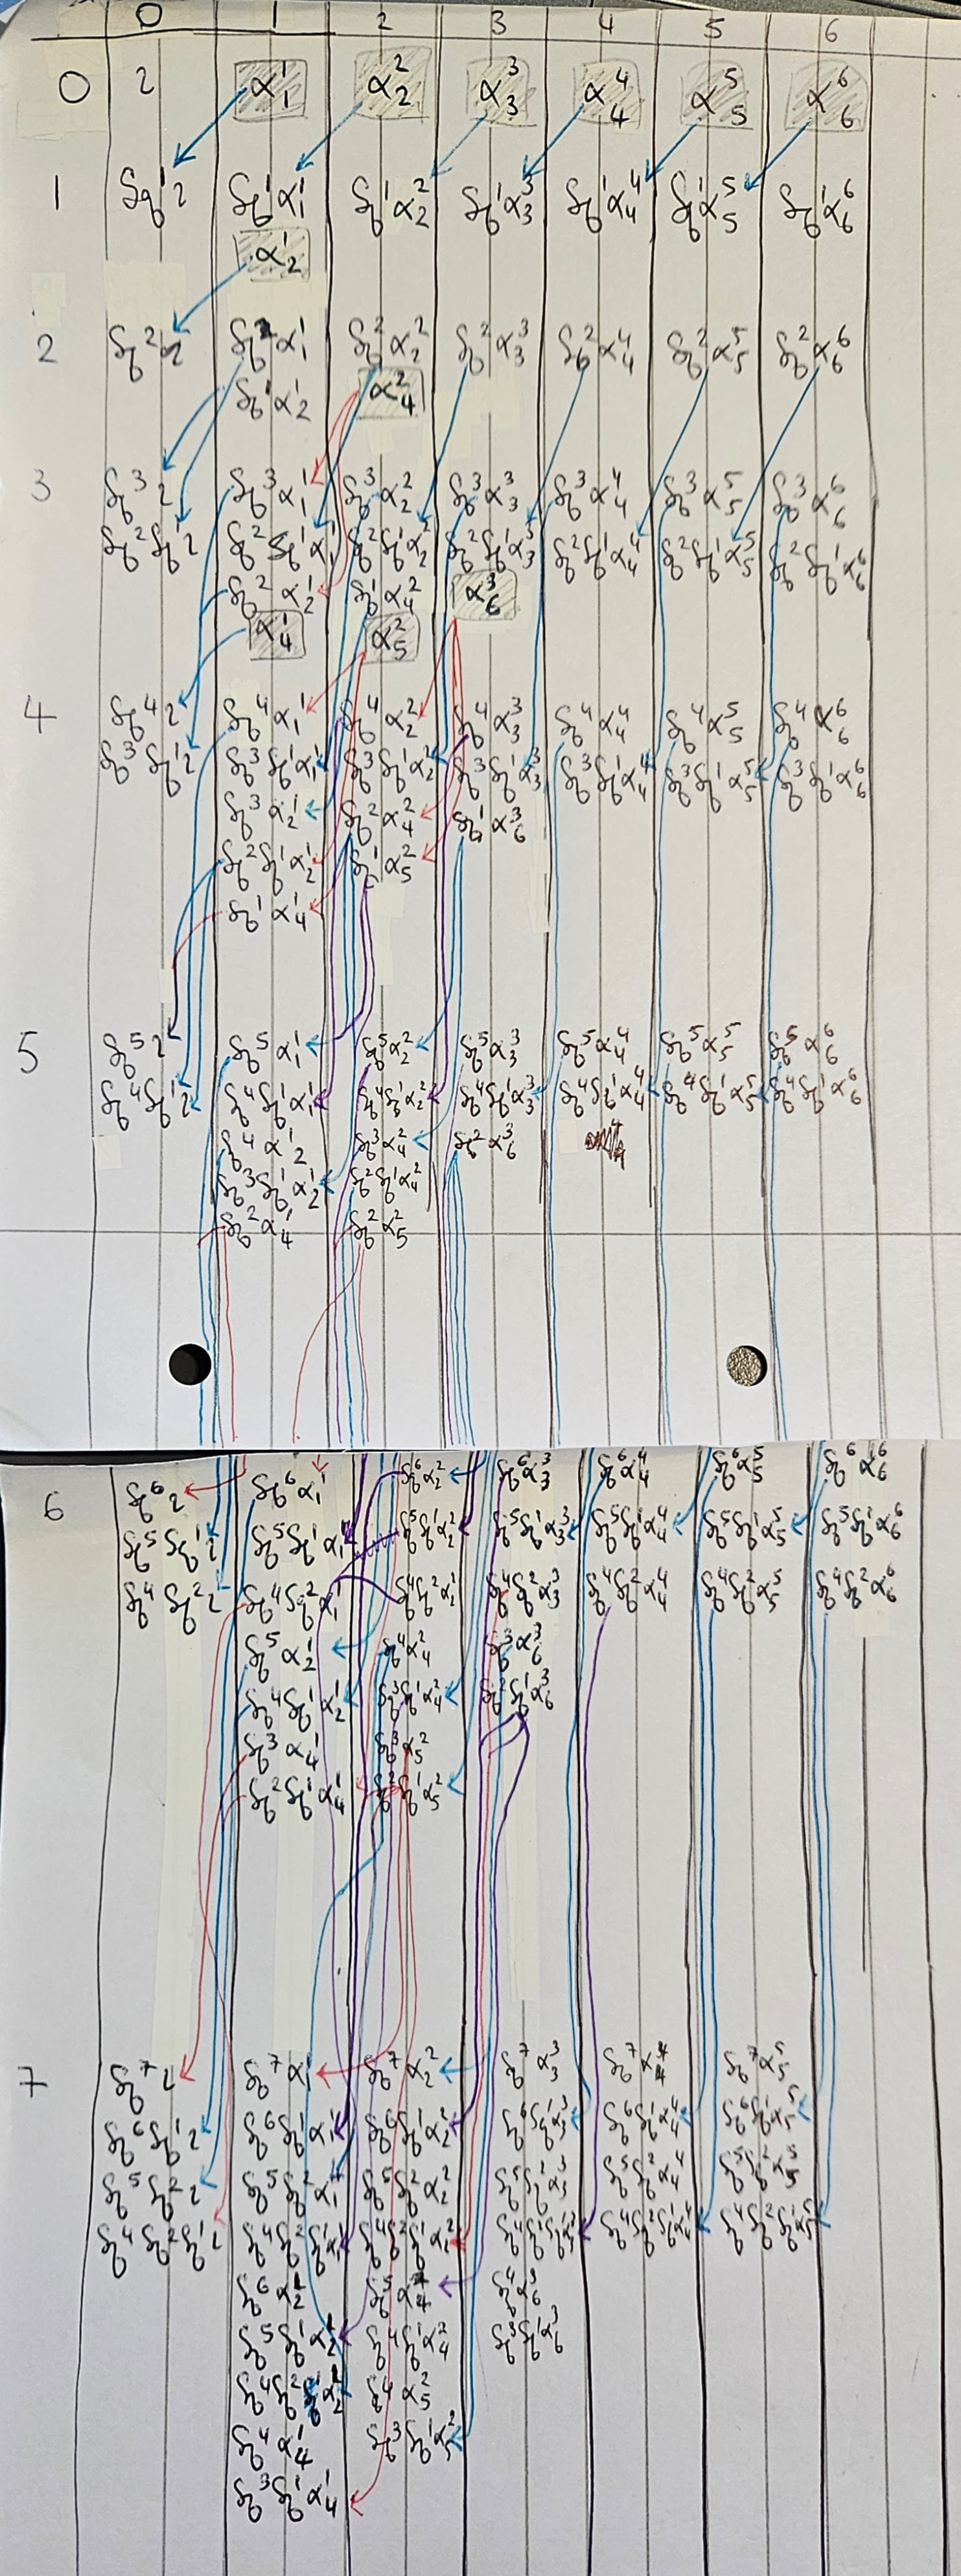
\includegraphics[width=0.4\textwidth]{ext3}
\caption{Calculating the first 5 rows}
\end{figure}

\begin{lemma}
There are no nontrivial differentials for \(t-s\leq 13\). 
\end{lemma}

\begin{ourproof}
First, note that the only possible nontrivial differentials in this range are \(d_r : E_r^{1,2} \to E_r^{1+r, 1+r}\) and \(d_2 : E_2^{2, 10} \to E_2^{4, 11}\). 

Now, \(0=d_r(h_0h_1)=d_r(h_0)h_1 + h_0d_r(h_1)=h_0d_r(h_1)\), so \(d_r(h_1)=0\). Since \(E_r^{1, 2}\) is generated by \(h_1\), we must have \(d_r=0\). 

On the other hand, \(E^{2, 10}\) is generated by \(h_1h_3\), and \(d_2(h_1h_3)=d_2(h_1)h_3+h_1d_2(h_3)=0+0=0\) (the first factor is zero by the previous computation, and the second is an element of a trivial group). \done
\end{ourproof}

\textcolour{teal}{[Obviously justify the \(h\) notation and the claims above that the generators are what I say they are]}

\subsection{Resolving extensions}

%Some slightly less cryptic comments are made in \autocite{cobordism}, in particular stemming from Lemma 3.1.3. If I just believe this lemma for the moment, assuming its \(a_0\) is the same as my \(\alpha^1_1\), and further believe the calculations done in \autocite{ass} in 6.2, then (I think!) this solves my problems.]

\begin{proposition}[{\autocite{ass}, Cor 6.5}]
We have the following relations:
\begin{align*}
\alpha^i_i &= (\alpha_1^1)^i\\
\alpha_4^2&=(\alpha^1_2)^2\\
\alpha^2_5&=\alpha^1_1 \alpha^1_4\\
\alpha^3_6&=(\alpha^1_1)^2 \alpha_4^1=(\alpha^1_2)^3.
\end{align*}
\end{proposition}

A few other things:
\begin{enumerate}
\item We know that \(\pi_0^S=\inte\) since \(\pi_1S^1=\inte\) and \(n=1\leq 2=2(1)\), so this lies in the stable region. Now, \(E^{s,t}\) is actually supposed to converge to some filtration of \(\inte_2\) (i.e. the 2-adics) (i.e. \(\text{}_2\inte\)) I think? But either way, we know that for our filtration all the quotients are \(\inte/2\inte\). I claim\footnote{Here is an absolutely ridiculous argument for that: \((\inte_2, +)\) is a topological group. For any subgroup \(H\) of finite index \(n=2^km\), \(H\) is open (since by Lagrange's theorem \(n\inte_2\subq H\) and thus \(n\inte_2=2^k\inte_2\), so \(x+2^k\inte_2\) is an open ball around any \(x\in H\)). Now, every open subgroup of \(\inte_2\) is also closed (since it's complement is a union of open cosets), and it's apparently the case [elaborate] that the closed subgroups of \(\inte_2\) are the ideals \(2^k\inte_2\). These facts then imply that the filtration I give is the only possible one. Short answer: finite index subgroups of \(\inte_p\) are of the form \(p^k\inte_p\).} then that the filtration must be \(\cdots 4\inte_2 \subq 2\inte_2 \subq \inte_2\). 
\item If that's true then \(\iota=[1]\in \inte_2/2\inte_2\), and using the multiplication above we see \(\iota\) is a unit. We also have \(h_0=[2]\in 2\inte_2/4\inte_2\) so \(h_0=[2]=[2[1]]=[2\iota]\), so \(h_0\) acts on \(\iota\) by multiplication by 2.
\item Now, for any \(\kappa\in E^{s,t}_2\), \(h_0\cdot \kappa = (\iota h_0)\cdot \kappa=2\kappa\). 
\end{enumerate}
The notation's a bit weird above, when I say `multiplication by 2' I mean: take \(\kappa \in E^{s,t}=F^{s,t}/F^{s+1,t+1}\). Then \(2\kappa \in F^{s+1,t+1}\) since it's a bunch of \(\bb{F}_2\)'s. Take it's equivalence class to get an element of \(F^{s+1, t+1}/F^{s+2,t+2}\). That's what I really mean by \(2\kappa\) and it's in \(E^{s+1,t+1}\).

All this is to say if I start multiplying higher things by \(h_0\), that \textit{is} multiplying by 2. So I can start resolving extensions this way.]

%[Should I even have the below as a proposition? Should I cite \autocite{cobordism}? His \(a_0\) is defined completely differently to my \(\alpha^1_1\) and his proof uses some sort of naturality? I think my explanation aligns much more closely with \autocite{ass} or \autocite{rognes2}.]

%\begin{proposition}[{\autocite{cobordism}, Lem 3.1.3(b)}]
%If \(x \in \Ext^{s,t}(\bb{F}_2, \bb{F}_2)\) is a permanent cycle in the Adams spectral sequence represented by \(\alpha \in \pi_*^S\), then \(\alpha^1_1x\) is a permanent cycle represented by \(2 \alpha\). 
%\end{proposition}

\textcolour{violet}{[Justify the below with sseq, not quite sure how to do this in a satisfying way though. See note in Section \ref{2503221342}]}

\begin{theorem}
\begin{align*}
\text{}_{2}\pi_i^S = \begin{cases}
\inte/2\inte & i = 1, 2, 6,10\\
\inte/8\inte & i = 3, 11\\
0 & i = 4, 5, 12, 13\\
\inte/16\inte & i = 7\\
(\inte/2\inte)^2 & i = 8\\
(\inte/2\inte)^3 & i=9.
\end{cases}
\end{align*}
\end{theorem}

\subsection{Nontrivial differentials}

[The point here is that all differentials interacting with \(E^{s,t}\) for \(t-s=14\) are trivial, and thus computing the stable homotopy groups is purely mechanical, because everything that appears on this part of the \(E_2\) page has to survive to \(E_\infty\). Thus, the `ambiguity' at \(t-s=14\) is just the fact that this is the first time you need to actually compute differentials.

\begin{enumerate}
\item The \(d_2\) differential at \(E^{1, 16}_2\) is nontrivial: \autocite{rognes2}, Thm 11.10.2:
\begin{itemize}
\item \textcolour{teal}{\(h_0\) detects\footnote{Make precise.} \(2 \in \text{}_2\pi^S_0\).}
\item \(h_3\) detects some \(\sigma \in \text{}_2\pi^S_7\).
\item \textcolour{teal}{By multiplicativity [?] \(h_0h_3^2\) detects \(2 \sigma^2\). }
\item \(\text{}_2\pi_*^S\) is graded commutative.
\item Thus, \(\sigma^2=-\sigma^2\), so \(2 \sigma^2=0\).
\item Thus, \(h_0h_3^2=0\) in \(E_\infty\), so it is the boundary of a differential. The only possibility is \(d_2(h_4)=h_0h_3^2\). 
\end{itemize}
\item \textcolour{violet}{The \(d_3\) differential at \(E^{2, 17}_3\) is nontrivial: \autocite{rognes2}, Thm 11.10.7 (which he doesn't prove, so really it's \autocite{rognes2} Table 14.2 (10), which uses a differential \(d_2\) of \(E_2(C\sigma)\) which is on table 14.9 (4)(!)).} 
\end{enumerate}

\autocite{stable_homotopy}, \autocite{cobordism}, \autocite{ass}, \autocite{rognes2}.

\appendix 

\section{Algebra}

\subsection{Free resolutions}\label{2502220958}

\begin{definition}
Let \(M, N\) be modules over a ring \(R\). A \textit{resolution} \(F\) of \(M\) is an exact sequence 
\[\cdots \to F_2 \to F_1 \to F_0 \to M \to 0.\]
If in addition each \(F_i\) is a free \(R\)-module, then the resolution is called \textit{free}. 
\end{definition}

Given a free resolution as above, applying \(\Hom_R(-, N)\) gives us a chain complex
\[\cdots \leftarrow \Hom_R(F_2, N) \leftarrow \Hom_R(F_1, N) \leftarrow \Hom_R(F_0, N) \leftarrow \Hom_R(M, N) \leftarrow 0.\]
Dropping the term \(\Hom_R(M, N)\) [why?] we get the sequence
\[\cdots \leftarrow \Hom_R(F_2, N) \leftarrow \Hom_R(F_1, N) \leftarrow \Hom_R(F_0, N) \leftarrow 0,\]
and we define \(\Ext^n_R(M, N)\) to be the \(n\)th homology group of this chain complex. 

%we write \(H^n(F; G):=\ker f^*_{n+1}/\im f_n^*\). Any abelian group \(H\) has a free resolution of the form 
%\[0 \to F_1 \to F_0 \to H \to 0\]
%(the one you think it is). So we get a chain complex
%\[0 \leftarrow F_1^* \leftarrow F_0^* \leftarrow H^* \leftarrow 0.\]
%We have \(H^n(F; G)=0\) for \(n>1\). Define \(\Ext(H;G):=H^1(F;G)\). 

\textcolour{teal}{[these do not depend on the choice of free resolution of \(M\)]}

A free resolution is \textit{minimal} if at each stage of its construction we choose the minimal number of free generators for \(F_i\) in each degree.

[The above definition is bad but I'm keeping it just for the moment.]

\subsection{Completion of abelian groups}

\begin{definition}[{\autocite{concise}, Def 10.1.1}]
Let \(A\) be an abelian group. Then its \textit{\(p\)-adic completion} is the limit 
\[\text{}_pA=\lim\limits_{\leftarrow n} (A/p^nA).\]
\end{definition}

If \(A=\inte\), we instead write \(\inte_p\) for the \(p\)-adic integers.

There is a natural map \(A \to \text{}_pA\), whose component at \(n\) is reduction modulo \(p^nA\). 

[\autocite{concise} p154]:

?When \(A\) is finitely generated, its \(p\)-adic completion is given by the map \(A \to A\otimes \inte_p\); \(a\mapsto a\otimes 1\). 

\begin{lemma}\label{2504031247}
Suppose \(A\) is finite, and write \(\abs{A}=np^r\) for \(p\nvert n\). Then \(A\otimes\inte_p\cong A/T\), where \(T\subq A\) is the subgroup generated by all torsion coprime to \(p\).
\end{lemma}

\begin{ourproof}
Define a homomorphism \(A\otimes\inte_p\to A/T\) sending \(a\otimes z \mapsto [q(z)a]\), where \(q\) is the projection \(\inte_p \surj \inte/p^r\inte\). Suppose \(a\otimes z\mapsto 0\). Then \(q(z)a\in T\), so \(kq(z)a=0\) for some \(k\) coprime to \(p\), and thus \(q(z)a\otimes z=kq(z)a\otimes \frac{1}{k}z=0\). On the other hand, \(z=q(z)z'\) for some \(z'\in \inte_p\), so \(a\otimes z = q(z) \otimes z'\). Thus, \(a\otimes z = 0\), so the map is injective. The map is clearly also surjective, since \(a\otimes 1 \mapsto [a]\), so it is an isomorphism. \done
\end{ourproof}

\section{Topology}

All from \autocite{hatcher} unless otherwise stated.

\subsection{Suspension}

\begin{definition}
Let \(X\) be a topological space. The \textit{suspension} \(SX\) is the space \newline\((X\times I)/\sim\), where \((x, 0)\sim (x', 0)\) and \((x,1)\sim (x',1)\) for all \(x,x'\in X\). 
\end{definition}

\begin{definition}
Let \(X\) be a pointed topological space. The \textit{reduced suspension} \(\Sigma X\) is the space \(SX/\sim\), where \([x_0, t]\sim [x_0, t']\) for all \(t,t'\in I\). 
\end{definition}

Given a map \(f : X \to Y\), we can define \(\Sigma f : \Sigma X \to \Sigma Y\) by \(\Sigma f[(x, t)]=[(fx, t)]\). This makes \(\Sigma \) into a functor \(\Sigma : \textbf{Top}\to \textbf{Top}\). 

\begin{remark}\label{2502141442}
\(\Sigma\) is faithful, since for any maps \(f, g : X\to Y\), if \(\Sigma f = \Sigma g\) then in particular \([(fx, \frac{1}{2})]=[(gx, \frac{1}{2})]\), so \(fx=gx\). 
\end{remark}  

[below is reconstructed from  \autocite{mazelgee}]

Given pointed maps \(f, g : \Sigma X \to Z\), define 
\begin{align*}
f \star g : \Sigma X &\to Z\\
[x,t]&\mapsto \begin{cases}
f[x,2t-1] & t \geq \frac{1}{2},\\
g[x,2t] &t\leq \frac{1}{2}.
\end{cases}
\end{align*}
This is well defined, since both \(f\) and \(g\) are basepoint-preserving. %\(f[x,0]=f[x_0,0]=y_0=g[x_0,1]=g[x,1]\). Essentially, it's just because the maps are basepoint-preserving, and \([x,0]\) and \([x,1]\) are both just the basepoint.

\begin{remark}
This defines a group structure on \([\Sigma X, Z]\), and thus \([\Sigma^i X, Z]\) is a group for all \(i\geq 1\). For \(i\geq 2\), these can be shown to be abelian, via the Eckmann-Hilton argument.
\end{remark}

\begin{remark}\label{2502200937}
The homotopy groups \(\pi_i(Z)\) are a special case of the above construction, taking \(X:=S^{i-1}\). 
\end{remark}

%[There are two possible products on \([\Sigma^2 X, Z]\), and some variation on the Eckmann–Hilton argument works its magic to show it's actually commutative (and, apparently, automatically associative). ]

\begin{itemize}
\item Loops; the adjunction \(\Sigma \dashv \Omega\), where \(\Omega\) is the loop functor.
\end{itemize}

\autocite{hatcher}, p395:

\begin{remark}
It follows that \(\pi_{n+1}(X)\cong \pi_n(\Omega X)\). In particular, \(\Omega K(G, n)\) is a \newline\(K(G, n-1)\). 
\end{remark}

\begin{itemize}
\item \autocite{hatcher} 2.1 Ex 20 and 2.2 Ex 32: \(\widetilde H_n(X)\cong \widetilde H_{n+1}(SX)\), where \(S\) is the (non-reduced) suspension.  (MV?) 
\item Hatcher also says on p219 that \(\widetilde H^n(X;R)\cong \widetilde H^{n+k}(\Sigma^kX;R)\), where \(\Sigma \) is reduced suspension.
\end{itemize}

\subsection{Other basic constructions}

\begin{definition}
Let \((X, x_0), (Y, y_0)\) be pointed topological spaces, and consider their product \(X\times Y\). The subspaces \(X\times\{y_0\}\cong X\) and \(\{x_0\}\times Y\cong Y\) intersect at exactly one point, \((x_0, y_0)\), and so can be identified with the wedge \(X\vee Y\). We thus define the \textit{smash product} \(X\wedge Y:=(X\times Y)/(X\vee Y)\), with the canonical basepoint \((x_0,y_0)\).  
\end{definition}

\begin{example}
We have \(S^n \wedge S^m\cong S^{n+m}\). \textcolour{teal}{[is this obvious?]}
\end{example}

\begin{remark}
Note that \(\Sigma X \cong X\wedge S^1\). 
\end{remark}

\begin{remark}\label{2503311142}
Observe that \(X\wedge (Y\wedge Z)\cong (X\wedge Y)\wedge Z\). Combining this with the remarks above, we see that \(\Sigma^kX\cong X\wedge S^k\). 
\end{remark}

\begin{remark}\label{2502211505}
Note that \(\Sigma(X\vee Y)\cong \Sigma X\vee \Sigma Y\).
\end{remark}

\begin{itemize}
\item The Eilenberg-MacLane space is \(K(G, n)\), and it has the property that 
\[\pi_i(K(G, n))=\begin{cases}
G & i=n,\\
0 & i\neq n.
\end{cases}\]
They're unique up to weak homotopy equivalence (i.e. if you have another one \(X\), there's a map between them which descends to an isomorphism on homotopy groups). They can be taken to be CW complexes. 
\end{itemize}

\begin{definition}
Let \(X\), \(Y\) be topological spaces, where \(X\) has a basepoint \(x_0\). Then the \textit{reduced product} \(X\times_{\text{red}}Y:=(X\times Y)/(x_0 \times Y)\). 
\end{definition}

\begin{definition}
Let \(f : X \to Y\) be a map. The \textit{mapping cylinder} \(M_f\) is defined by \(((X\times I)\sqcup Y)/\sim\), where \((x,1)\sim f(x)\) for all \(x \in X\). If \((X, x_0), (Y, y_0)\) are pointed spaces, the \textit{reduced mapping cylinder} is the quotient \(M_f/\sim\), where \([x_0, t]\sim [x_0, t']\) for all \( t\in I\).
\end{definition}

\begin{remark}\label{2503231306}
The mapping cylinder deformation retracts onto \(Y\) via \(h : M_f \times I\to M_f\); \(([x,t], s)\mapsto [x, t+s(1-t)]\). 
\end{remark}

\begin{definition}
Let \(f : X \to Y\) be a map. The \textit{mapping cone}\footnote{Why does Hatcher not insist this guy is reduced, like he does with the mapping cylinders?} \(C_f\) is defined to be \(Y\sqcup_f CX:=(Y\sqcup CX)/(f(x)\sim [x,1])\). 
\end{definition}

\subsection{Cell complexes}\label{2502141508}

\begin{definition}
Let \(X\) be a cell complex, \(A\subq X\) a subcomplex. Then the quotient \(X/A\) has a cell complex structure, with cells the cells of \(X\setminus A\) along with a basepoint (the image of \(A\) in \(X\)). 
\end{definition}

\begin{definition}
Let \(f : X \to Y\) be a map between CW complexes. Then \(f\) is \textit{cellular} if \(f(X_{(n)})\subq Y_{(n)}\) for all \(n\), where \(X_{(n)}\) is the \(n\)-skeleton of \(X\). 
\end{definition}

Cellular approximation theorem:

%might not even need this but it looks useful
\begin{theorem}[{\autocite{hatcher}, Thm 4.8}]\label{2502211420}
Let \(f : X \to Y\) be a map of CW complexes. Then \(f\) is homotopic to a cellular map.
\end{theorem}

\begin{lemma}[{\autocite{hatcher}, Prop 0.16}]\label{2502211419}
Let \(A\subq X\) be CW complexes. Then the pair \((X, A)\) has the \textit{homotopy extension property}; that is, for any map \(f : X \to Y\) and homotopy \(h : A\times I \to Y\) such that \(h(a,0)=f|_A\), there is a homotopy \(\widetilde h : X\times I \to Y\) extending \(h\). 
\end{lemma}

\begin{itemize}
\item The product of cell complexes is a cell complex (maybe only if one of them is finite?)
\item The smash product of (pointed?) cell complexes is a cell complex (maybe only if one is them is finite?) [\autocite{hatcher} says ``the smash product \(X\wedge Y\) is a cell complex if \(X\) and \(Y\) are cell complexes with \(x_0\) and \(y_0\) \(0\)-cells, assuming that we give \(X\times Y\) the cell-complex topology rather than the product topology in cases where these two topologies differ''.]
%\item The reduced suspension of a pointed cell complex is a pointed cell complex.
%\item CW pairs? [they're literally just pairs of some CW complex and a subcomplex]
\item For a CW complex \(X\), \(SX\simeq \Sigma X\).
\item The reduced suspension of a pointed cell complex \((X, x_0)\) is another pointed cell complex \(\Sigma X\) with basepoint \(x_0\) and an \(n\)-cell for each non-basepoint \(n-1\) cell \(e^{n-1}_\alpha\) of \(X\).
\end{itemize}

\begin{definition}
Let \(X\) is a topological space. A \textit{CW approximation} to \(X\) is a CW complex \(Z\) equipped with a weak homotopy equivalence \(f : Z \to X\).
\end{definition}

\begin{theorem}[{\autocite{hatcher}, Prop 4.13}]
Every space \(X\) has a CW approximation \(f : Z \to X\). %If \(X\) is path-connected, \(Z\) can be chosen to have a single 0-cell, with all other cells attached by basepoint-preserving maps. 
\end{theorem}

\begin{itemize}
\item In particular, \(\Omega K(G, n)\) has a CW approximation \(Z \to \Omega K(G, n)\), and since \(\Omega K(G,n)\) is a \(K(G,n-1)\), so is \(Z\). 
\item Something along the lines of `compact \(\leftrightarrow\) finite number of cells'.
\end{itemize}

\section{Notes to self}\label{C}

\subsection{Vague problems and questions....}

\subsubsection{...that probably don't matter}

\begin{itemize}
%\item Is `pointed' (co)homology just reduced (co)homology? I've noticed `pointed things' (\(\Sigma, \Omega, \wedge\), ...) seem to happen to/in reduced (co)homology, and `unpointed things' (\(S, \times, ...\)) happen to/in normal (co)homology. I want to do pointed things. 

%\item What does Hatcher mean when he says two spectra are `equivalent'? (usual definition of sameness)

\item On p588 of \autocite{hatcher5}, he says ``every CW spectrum is equivalent to a suspension spectrum''. Does he actually mean that, or does he mean `equivalent to the suspension of a spectrum'? The former seems way too strong, although in fairness I still don't know what an equivalence of spectra actually \textit{is}. 

%\item Suppose I have the \(E_2\) page for the appropriate spectral sequence. That in principle only gives me the `dots' and possibly the differentials. But if I just want to calculate, say, \(\pi^S_3\), I get \(\inte_2\) summands at \(E^{1, 4}_2, E^{2, 5}_2,\) and \(E^{3, 6}_2\). So, that says I have a filtration 
%\[0 \subq \inte_2 \subq F^{2,5}\subq F^{1,4}=\pi^S_3,\]
%and \(F^{2,5}/\inte_2\cong \inte_2\), \(F^{1,4}/F^{2,5}\cong \inte_2\). So \(\pi^S_3\) has order 8 and a filtration by \(\inte_2\)'s, but that still doesn't tell me whether it's \(\inte_8, \inte_4\times \inte_2\) or \(\inte_2^3\)? Thm 5.47 of \autocite{hatcher5} tells me that \(F^{s,t}\) is the image of the map \(\pi_t(\bb{S}_s)\to \pi_3^S\), so do I have to go back to the constructing and figure out what that map actually is, or is there something algebraic I can do?\footnote{I think this related to something \autocite{ass} calls the Yoneda product on p47-50 and 61-62 - this is a multiplicative structure on \(E_2\) and should tell me something about the additive structure of \(\pi_*^S\).}

\item On p586 of \autocite{hatcher5}, Hatcher says ``If \(X\) is of finite type then for each \(i\) there is an \(n\) such that \(X_n\) contains all the \(i\)-cells of \(X\). It follows that \(H_i(X;G)=H_i(X_n;G)\) for all sufficiently large \(n\), and the same is true for cohomology.'' But from the way he set up \(H_*\) and \(H^*\) earlier, shouldn't this be \(H_i(X;G)=H_{i+n}(X_n; G)\)? Because \(H_i(X;G)=\lim\limits_{\rightarrow}H_{i+n}(X_n)\), and he talks about things stabilising in the next sentence, so shouldn't the stable point be at some \(H_{i+n}\)?

\item I write \(\A\) where Hatcher writes \(\mathscr{A}\). We mean the same thing, right...?

\end{itemize}

\subsubsection{...that probably do matter}\label{2504011259timeforlunchithink}

\begin{itemize}
\item I am definitely being told some lies about what the spectral sequence actually converges to. There's a strong implication/actual statement(!!) that at each \(i\) it's supposed to be a filtration of \(\pi_i^S\) modulo odd torsion, but I think this isn't true. I think it's actually the 2-completion of \(\pi_i^S\). That coincides with the \(p\)-primary part for finite abelian groups, but for \(\pi_0^S\) it's supposed to be \(\inte_2\) (i.e. the 2-adic integers), not \(\inte\). I believe. Maybe get a source for this. Some people say it's the localisation at 2?? But I think that's also a lie. 

\item The Leibniz rule is \(d_r(xy)=d_r(x)y\pm xd_r(y)\) (can't remember the sign). But anything I'm using that rule on is some generator of an \(\bb{F}_2\), right? So the sign shouldn't matter. But then, shouldn't the Yoneda product be graded commutative (and thus commutative, because again, in the target signs don't matter)? So why does \autocite{ass} have some comment (in Cor 6.5) about how the Yoneda product is commutative ``in [some] range''?? 

\item On p592 of \autocite{hatcher5}, he says that ``for spectra \(X\) of finite type [the more general] definition of an \(\A\)-module structure on \(H^*(X)\) agrees with the definition using the usual \(\A\)-module structure on the cohomology of spaces and the identification of \(H^*(X)\) with the inverse limit \(\lim\limits_{\leftarrow}H^{*+n}(X_n)\)''. Um? Sure, we have that each \(H^{i+n}(X_n)\) stabilises eventually, but is Hatcher saying \(H^{*+n}(X_n)\) stabilises? Like, as an \(\A\)-module? And if not, what's going on here? Because inverse limits don't commute with infinite direct sums - they're not biproducts anymore, they're coproducts and there's no reason limits should commute with them. 

\item There's something weird going on with products. So, things are ok in \textbf{Top}, because we have the ordinary product of two spaces, which is a categorical product. But with CW complexes, supposedly sometimes the product topology differs from the `cell complex topology'? But, regardless, we're supposed to be working with pointed things - so in \(\textbf{Top}_*\), the pointed coproduct is the wedge sum, and the pointed product is just the normal product \(X\times Y\) with the basepoint \((x_0,y_0)\) (it's not the smash product). But what about in spectra? No one ever seems to talk about products of spectra, but for example a collection of maps \(X\to \bb{K}(G,n_i)\) should correspond to a single map \(X\to \prod_i \bb{K}(G,n_i)\), whatever that last object is. 

The plot thickens. From \href{https://ncatlab.org/nlab/show/Eilenberg-Mac+Lane+spectrum}{the nLab}: ``[some smash product] is non-canonically equivalent to a product of EM-spectra (hence a wedge sum of EM-spectra in the finite case)''. ???????

\item Question: so I have this multiplicative structure on the entire spectral sequence, right? And on the second page it's just the Yoneda product. But say I compute, I don't know, \(\alpha^2_5=h_0h_2\) on the \(E_2\)  page. Since none of those guys are touched by differentials, is that computation still valid on the \(E_3\) page? And on higher pages?
\end{itemize}

\subsection{To do}\label{2503221342}

Now:

\begin{itemize}
%\item Find out what the deal with reduced cohomology and being stable under suspension is. % It's just the fact that \wildetilde{H}_i(X) \cong \widetilde{H}_{i+1}(\Sigma X). More interesting is *which* isomorphism we're using here...
\item Find out what the ``suspension isomorphism given by reduced cross product with a generator of \(H^1(S^1; \bb{F}_2)\)'' is. 

\item Find out what the \(\bb{F}_2\) Bockstein homomorphism is.

\item Write down the induced maps on \(\pi_*\) and \(H^*\)/\(H_*\) from maps of spectra.

\item Check composition of maps of spectra is well-defined.

\item Prove that a spectrum is equivalent to the suspension of some other spectrum.

\item Prove that \([X,Y]\) is an abelian group for \(X,Y\) spectra.

\item Prove that the suspension map \([X,Y]\to [\Sigma X, \Sigma Y]\) is a group isomorphism. 

\item Derive the exact sequence
\[[Y,A]\to [Y,X]\to [Y, X/A]\to [Y, \Sigma A]\to [Y, \Sigma X].\]

\item Rewrite Sections \ref{2504041910} and \ref{2503301333} and fix the grading.

\item Show the action of \(\A\) on \(H^*(X)\) is actually a module action.

\item Figure out the whole wedge/product of EM spectra nonsense and why \(K_0\) has finite type. 

\item Figure out when and why maps can be replaced by inclusions.

\item Figure out why applying \(H^*\) to the sequence \(k_0\to K_1 \to \cdots\) makes it exact.

\item Show that the \(H*(K_s)\)'s are free \(\A\)-modules.

\item Show that there is a natural map \([\bb{S}, K_s]\to \Hom^0_{\A}(H^*(K_s), H^*(\bb{S}))\), and that it's an isomorphism (Yoneda?). 

\item Find out how much of this you should be proving.

\item Explain the Yoneda product at all coherently, and compute some examples.

\item Prove that \(\pi_*^S\) is a graded commutative ring.

\item Find out where the universal property of \(p\)-completion comes from. 

\item Find a way to translate the calculations in \ref{2504041920} into readable and coherent LaTeX'd calculations, and make some figures of pages of the spectral sequence (up to 14 I guess..) 

\item Make the \(\alpha^i_j\) notation not appalling - link it to the usual \(h\) notation.

\item Make the language of `detection' precise. 

\item Prove that the \(d_3\) differential at \(E^{2,17}\) is nontrivial.
\end{itemize}

Eventually:

\begin{itemize}
\item Be consistent with either cell complex or CW complex.

\item Be consistent with \(\bb{F}_2\)  or \(\inte/2\inte\) (don't use \(\inte_2\), that's really bad).

\item Specialise the Adams spectral sequence (i.e. set \(Y=\bb{S}\)).

\item Remember that you have to hand in the tex file, so for the love of god change anything stupid that's hidden in the pdf.

\item Sometimes I say \(\pi_*^S\) or \(\text{}_{(2)}\pi_*^S\) (localised at 2?) instead of its completion at 2 or whatever. So make sure it's correct.

\item Stick to a convention on suspension/cone/homotopy numbering. I.e. Does a homotopy start at 0 or 1? Does a suspension go from -1 to 1 with the space in the middle at 0, or 0 to 1 with the space at \(1/2\)? Do cones go from 0 to 1, and if so, make sure when they include into suspensions they do so consistently. 

\item I want to at some point compute \(h_0h_1h_3\) or something like that, just to show that sometimes a product can be zero even if it lands in a nonzero group (i.e. the stable groups aren't all cyclic). The trouble is by the time you get to \(\pi_8^S\) the free resolution is an awful mess. Maybe I can try and wrangle with the sseq program to get it to show me kernels and the like?

\item Ease notation by not writing \(G\) in e.g. \(H^*(X;G)\). Say we're taking coefficients in \(\bb{F}_2\), but actually a lot of the time it doesn't matter so maybe note that.

\item Have any sort of consistency in using or not using brackets (e.g. \(\pi_t X_s\) v.s. \(\pi_t(X_s)\)). 

\item When I say `spectrum' at any point after defining CW spectra I mean `CW spectrum'. And I basically always mean `connective CW spectrum of finite type' too. 

\end{itemize}

\subsection{Other notes}\label{2503231313}

\begin{itemize}
\item READ IF YOUR CALCULATIONS AREN'T WORKING: You are working modulo 2!!!

\item If you have a bunch of maps between graded modules/algebras, they're graded homomorphisms. So they preserve degree. 

\item All (co)homology is supposed to be reduced.
%\item On p592 of \autocite{hatcher5}, he says that ``for spectra \(X\) of finite type [the more general] definition of an \(\A\)-module structure on \(H^*(X)\) agrees with the definition using the usual \(\A\)-module structure on the cohomology of spaces and the identification of \(H^*(X)\) with the inverse limit \(\lim\limits_{\leftarrow}H^{*+n}(X_n)\)''. Absolutely everything relevant to spheres in the construction of the Adams spectral sequence seems to only use spectra of finite type, but Hatcher says on p585 that we can't just take the inverse limit because it doesn't work for the `more general spectra' used when constructing the Adams spectral sequence. I believe this is because the Adams spectral sequence is defined for \(X\) not of finite type, though Hatcher only constructs it for finite type guys.
\item Signs don't matter with the Leibniz rule either!! You are working modulo 2!!!!!!!!

\item Remember, once you know that \(d_2(h_4)=h_0h_3^2\), you know \(h_4\) \textit{doesn't survive to the third page}. So, for example, \(d_3(h_0h_4)\neq h_0d_3(h_4)\) because \(h_4\) doesn't exist anymore. That's why \(d_3(h_0h_4)\) can be nonzero. 

\item As previously mentioned, we are working modulo 2!! What this also implies is that if anything is hit by any sort of differential, or has any nonzero differential coming out of it, it's completely killed by the next page. Because the summands are just a bunch of \(\bb{F}_2\)'s (so you don't need to worry about `how much' of something is killed, it all is). 

\item Sometimes Hatcher says that you can replace any map of CW complexes by an inclusion. I think the point here is that if you have a map \(f : X \to Y\), \ref{2503231306} says that \(M_f\) deformation retracts onto \(Y\). So if you only care about \(X\) and \(Y\) up to homotopy equivalence, you can replace \(Y\) by \(M_f\) and then \(X\) definitely includes into \(M_f\). 

\item Where it's ambiguous, I'm marking things I definitely need by ! and things I think I may not need by ?.

\item By the way, the argument at footnote 11 looks a little unsettling, because it seems like you could use it to show that \textit{all} homotopy groups are trivial eventually. And that's true! But when you take the colimit \(\pi_i(X)=\colim_n \pi_{i+n}X_n\), notice that it's over \(\pi_{i+n}\), not \(\pi_{i}\). So yes, the connectivity of \(X_n\) increases with \(n\), but the index of \(\pi\) also does. Basically, it's all fine. I'm putting this note here because I will invariably forget this and have a heart attack a day before this is due thinking everything is broken. 

\item In literature, \(A^\wedge_p\) is the \(p\)-adic completion of \(A\). Sometimes I'll write this as \(\text{}_pA\) because of some stupid notational decisions I made earlier.

\item The `abutment' of a spectral sequence apparently means the thing it converges to (i.e. if \(E_\infty\) computes the associated graded of some \(H^*\), the abutment of \(\{E\}\) is \(H^*\) (not its associated graded)). 
\end{itemize}

Sources I've used: \autocite{cobordism}, 
\autocite{ass}, \autocite{spectra}, \autocite{hatcher5}, \autocite{hatcher}, \autocite{rognes2}, \autocite{concise}, \autocite{spectral_sequences}

Sources I probably won't use: \autocite{suspension}, \autocite{stable_homotopy}, \autocite{foundations}, \autocite{primer}, \autocite{mazelgee} (I think the construction I need is in Hatcher)

\printbibliography

\end{document}